\documentclass[journal]{IEEEtran}

% *** MISC UTILITY PACKAGES ***

\newcommand{\note}[1]{\textcolor{magenta}{#1}}

\usepackage{silence}
\WarningsOff[fixltx2e]

\usepackage[switch]{lineno}
\renewcommand{\linenumberfont}{\normalfont\bfseries\small\color{lightgray}}

% *** GRAPHICS RELATED PACKAGES ***
\usepackage{graphicx}
\graphicspath{{./figures/}}

% *** MATH PACKAGES ***
%% with other math-related packages, you may want to disable it.
\usepackage{amsmath, amsthm, amsfonts,amssymb,eulervm,xspace, mathtools}
\usepackage{stmaryrd}%maps from
%\renewcommand{\restriction}{\mathord{\upharpoonright}} %restriction w/p space
\usepackage{mathrsfs} % math script fonts
\usepackage{relsize} %bigger
\usepackage{bm}

% theorem environments
\theoremstyle{definition}
\newtheorem{definition}{Definition}[section]
\newcommand{\definitionautorefname}{Definition}
\theoremstyle{remark}
\newtheorem{example}{Example}[section]
\newtheorem{axiom}{Axiom}
\newtheorem{prop}{Proposition}

% *** diagrams
\usepackage{tikz}
\usetikzlibrary{cd}


% *** SPECIALIZED LIST PACKAGES ***
\usepackage{xcolor}
\usepackage[utf8]{inputenc}

\usepackage[outputdir=.]{minted}
\setminted[python]{fontsize=\scriptsize,
                   linenos,
                   numbersep=8pt,
                   frame=lines,
                   autogobble,
                   framesep=3mm,
                   breaklines=True}
% *** ALIGNMENT PACKAGES ***
\usepackage{multicol}
\usepackage{array}
\usepackage{multirow}
\usepackage{tabulary}
% IEEEtran contains the IEEEeqnarray family of commands

% *** SUBFIGURE PACKAGES ***
\usepackage[caption=false,font=normalsize,labelfont=sf,textfont=sf]{subfig}

% *** FLOAT PACKAGES ***
\usepackage{dblfloatfix}

% *** PDF, URL AND HYPERLINK PACKAGES ***
\usepackage{xurl}

% *** BIBLIOGRAPHY ***
\usepackage[]{footmisc}
\usepackage{bookmark}
\usepackage[style=ieee, backend=biber]{biblatex}
\addbibresource{references.bib}

%\usepackage[inline]{showlabels}

\usepackage{notation} %notation conventions
% correct bad hyphenation here
%\hyphenation{}

\begin{document}
\linenumbers

\title{Topological Equivariant Artist Model for Visualization Library Architecture}
% author names and IEEE memberships
\author{Hannah~Aizenman, Mikael Vejdemo-Johansson, Thomas~Caswell, and~Michael~Grossberg,~\IEEEmembership{Member,~IEEE,}% <-this % stops a space
\IEEEcompsocitemizethanks{\IEEEcompsocthanksitem H. Aizenman is with the department of Computer Science, The Gradaute Center, CUNY.
\protect\\
% note need leading \protect in front of \\ to get a newline within \thanks as
% \\ is fragile and will error, could use \hfil\break instead.
E-mail: haizenman@gradcenter.cuny.edu,
\IEEEcompsocthanksitem M. Grossberg is with the department of Computer Science, City College of New York, CUNY.
E-mail: mgrossberg@ccny.cuny.edu
\IEEEcompsocthanksitem Mikael Vejdemo-Johansson is with the department of Mathematics, CUNY College of Staten Island.
\protect\\
E-mail: mvj@math.csi.cuny.edu
\IEEEcompsocthanksitem Thomas Caswell is with National Synchrotron Light Source II, Brookhaven National Lab
\protect \\
E-mail: tcaswell@bnl.gov}% <-this % stops an unwanted space
\thanks{Manuscript received X XX, XXXX; revised X XX, XXXX.}
}


% for Computer Society papers, we must declare the abstract and index terms
% PRIOR to the title within the \IEEEtitleabstractindextext IEEEtran
% command as these need to go into the title area created by \maketitle.
% As a general rule, do not put math, special symbols or citations
% in the abstract or keywords.
\IEEEtitleabstractindextext{%
\begin{abstract}
  The contract data visualization tools make with their users is that a chart is a faithful and accurate visual representation of the numbers it is made from. Motivated by wanting to make better tools, we propose a methodology for fully specifying arbitrary data to visualization mappings in a manner that easily translates to code. We propose that fiber bundles provide a uniform interface for describing a variety of underlying data - tables, images, networks, etc. - in a manner that independently encodes the mathematical structure of the topology and the fields of the dataset. Modeling the data structures that store the datasets as sheaves provide a method for specifying visualization methods that are designed to work regardless of how the dataset is stored - whether the data is on disk, distributed, or on demand. Specifying the visualization library components as natural transforms of sheaves means that the constraints that the component must satisfy to be structure preserving can be specified as the set of morphisms on the data and graphic sheaves, including the structure on the topology and fields of the data.
  Using category theory to formally express how visual elements are constructed means we can translate those expectations into code, which can then be used to enforce the expectation that a visualization tool is faithfully translating between numbers and charts.
\end{abstract}

% Note that keywords are not normally used for peerreview papers.
\begin{IEEEkeywords}
%Computer Society, IEEE, IEEEtran, journal, \LaTeX, paper, template.
\end{IEEEkeywords}}


% make the title area
\maketitle
\IEEEpeerreviewmaketitle
\IEEEraisesectionheading{\section{Introduction}\label{sec:intro}}


\IEEEPARstart{V}isualization design guidelines, generally, describe how to choose visual encodings that preserve the structure of the data; to follow these guidelines the visualization tools that implement these $data \rightarrow graphic$ transforms must be structure preserving. Loosely, preserving structure means that the properties of the data and how the points are connected to each other should be inferable from the graphic such that a $graphic \rightarrow data$ mapping can be made. For example, values read off a bar chart have to be equivalent to the values used to construct that chart. Therefore a visualization tool is structure preserving when it preserves the bidirectional mapping $data\leftrightarrow graphic$.

We propose that we can better enforce this expectation in software by providing a uniform way of expressing $data$ and $graphic$ using their respective algebraic structure and by uniformly specifying the behaviors and properties of those structures and the maps between them using category theory. For example, our framework can encapsulate how a table and scatter plot and heatmap are different representations of the same data and track an observation from a data cube as a point along a time series and on a map and in a network. The algebraic structures can then be translated into programmatic types, while the categorical descriptions translate to a functional design framework. Strong typing and function composition enable visualization software developers to build complex components from simpler verifiable parts \cite{huHowFunctionalProgramming2015, hughesWhyFunctionalProgramming1989}. These components can be built as a standalone library and integrated into existing libraries and we hope these ideas will influence the architecture of critical data visualization libraries, such as Matplotlib.

The contribution of this paper is a methodology for describing structure, verifying structure preservation, and specifying the conditions for constructing a structure preserving map between data and graphics. This framework also provides guidance for the construction and testing of structure preserving visualization library components.

\section{Related Work}
\label{sec:related-work}

This paper builds on how structure has traditionally been discussed in visualization and mathematics and encapsulated in visualization library design to propose a uniform interface for encoding structure that supports a broader variety of fields and more rigorously define how connectivity is preserved. Generally, preserving structure means that a visualization is expected to preserve the $field$ properties and $topology$ of the corresponding dataset:

\begin{LaTeXdescription}
  \item[\textcolor{fiber}{\textbf{field}} \footnote{Throughout this paper, we use color in definitions, equations, and visualizations to group conceptually related terms\cite{headMathAugmentationHow2022}, for example \textcolor{fiber}{field} and \textcolor{fiber}{fiber}.}] is a set of values of the same type, e.g. one column of a table or the pixels of an image
  \item[\textcolor{base}{\textbf{topology}}] is the connectivity and relative positioning of elements in a dataset \cite{wilkinsonGrammarGraphics2005}.
\end{LaTeXdescription}

The conditions under which $data \rightarrow graphic$ is structure preserving is discussed extensively in the visualization literature, codified by Bertin\cite{bertinSemiologyGraphicsDiagrams2011} and extended to tool design by Mackinlay\cite{mackinlayAutomaticDesignGraphical1987}, and a set of conditions under which the $graphic \rightarrow data$ mapping is structure preserving is presented in Kindlemann and Scheidegger's algebraic visualization design (AVD) framework \cite{kindlmannAlgebraicProcessVisualization2014}. Encapsulating the AVD conditions, we present a uniform abstract data representation layer in \autoref{sec:atct:sheaves} for ensuring that the visualization should not change if the data representation (i.e. the data container) changes, define the conditions under which data is mapped unambiguously to visual encodings \cite{ziemkiewiczEmbeddingInformationVisualization2009} in \autoref{sec:atct:xi}, and provide a methodology for verifying that changes in data should correspond to changes in the visualization in \autoref{sec:artist:equivariant:artist} that does not necessarily require that the changes be perceptually significant. Furthermore, our model generalizes the AVD notion of equivariance by allowing non-group structures, explicitly incorporating topology and by providing a framework for translating the theoretical ideas into buildable components in \autoref{sec:construction}.

\subsection{Fields}
\label{sec:related-work:equivariance}

Data is often described by its mathematical structure, for example the Steven's measurement scales define nominal, ordinal, interval, and ratio data by the allowed operations on each \cite{stevensTheoryScalesMeasurement1946} and other researchers have since expanded the scales to encapsulate more types of structure \cite{leaFormalizationMeasurementScale1971, thomasMathematizationNotMeasurement2014}.

Loosely, the scales classify data as a set of values and the allowed transformations on that set, which can be operations, relations, or generalized as actions:

\begin{definition}\label{def:related-work:action}\cite{grimaldiDiscreteCombinatorialMathematics2006}
  An \textcolor{action}{\textbf{action}} of \textcolor{action}{$G = (G,\circ, e)$} on $X$ is a function  $act: \textcolor{action}{G} \times X \rightarrow X$. An action has the properties of identity $act(\textcolor{action}{e}, x) = x$ for all  $x \in X$ and associativity $act(\textcolor{action}{g}, act(\textcolor{action}{f}, x)) = act(\textcolor{action}{f} \circ \textcolor{action}{g}, x)$ for $\textcolor{action}{f},\textcolor{action}{g} \in \textcolor{action}{G}$.
\end{definition}

Elements of $X$ can be from one data field or all of them or some subset; similarly the actions act on
the elements of $X$ and each action can be a composition of actions. This means actions can be used when discussing various measures of structure preservation. For example, \textit{equivariant} functions preserve structure under transformations to data or visualization and has been proposed by Kindlemann and Scheidegger\cite{kindlmannAlgebraicProcessVisualization2014} and \textit{homomorphic} maps preserve relations between data elements was preserved as proposed by Mackinlay\cite{mackinlayAutomaticDesignGraphical1987}.

Specifically, Steven's conceptualizes the structure on values as \textcolor{action}{actions} on groups \footnote{A \textit{group} is a set with an associative binary operator. This operation must have an identity element and be closed, associative, and invertible}. A function that preserves structure when the input or output is changed by a group action is called \textit{equivariant}.

\begin{figure}
  \includegraphics*[width=1\columnwidth]{equivariant.pdf}
  \caption{Encoding data as the bar height using an exponential transform is not equivariant because encoding the data and then scaling the bar heights yields a much taller graph then scaling the data and then encoding those heights using the same exponential transform function.}
  \label{fig:related-work:equivariance}
\end{figure}

 Given a group $G$ that acts on both the input $X$ and the output $Y$ of a function $f: X \rightarrow Y$

\begin{definition}\label{def:equivariance}
 A function $f$ is \textbf{equivariant} when $f(act(g,x)) = act(g,f(x))$ for all $g$ in $G$ and for all $x$ in $X$ \cite{pittsNominalSetsNames2013}
\end{definition}
which means that a visualization is structure preserving when there exist compatible group actions on the data and visualization, as discussed by Kindlemann and Scheidegger\cite{kindlmannAlgebraicProcessVisualization2014}. As illustrated in the commutative diagram in \autoref{fig:related-work:equivariance}, what this means is that the visual representation is consistent whether the data is scaled and then mapped to a graphic or whether the data is mapped to a graphic that is then modified in a compatible way.

Although the Steven's scales were conceptualized as having group structure, the ordinal scale has a monoidal structure because partial orders ($\geq, \leq$) are not invertible. This means \textit{equivariance} cannot be used to test for structure preservation. Instead \textit{homomorphism} can be used because it imposes fewer constraints on the underlying mathematical structure of the data.
\begin{figure}
  \includegraphics[width=1\columnwidth]{homomorphism.pdf}
  \caption{Encoding data as bar height using an inverse transform is not homomorphic because the largest number is mapped to the smallest bar while the max function returns the largest bar.}
  \label{fig:related-work:homomorphism}
\end{figure}

Given the function $f: X \rightarrow Y$, with operators $(X, \circ)$ and $(Y, *)$

\begin{definition}\label{def:homomorphism}
  A function $f$ is \textbf{homomorphic} when $f(x_1 \circ x_2) = f(x_1) * f(x_2)$ and preserves identities $f(I_x) = I_y$ all $x, y \in X$ \cite{grimaldiDiscreteCombinatorialMathematics2006}
\end{definition}

which means that the operators $\circ$ and $*$ are compatible. In \autoref{fig:related-work:homomorphism}, the $\geq$ operator is defined as the compatible closed functions \texttt{max} and the inverse transform
is not homomorphic because it does not encode the maximum data value as the maximum bar value.

As shown in \autoref{fig:def:equivariance} and \autoref{fig:def:homomorphsim}, a function can be homomorphic but not equivariant, such as an exponential encoding, or equivariant but not homomorphic, such as the inverse encoding. A function can also be homomorphic (or equivariant) with respect to one action but not with respect to another. The encoding transforms in visualization tools are expected to preserve the structure of whatever input they receive; therefore a methodology for codifying arbitrary structure is presented in \autoref{sec:atct:fb:fiber} and \autoref{sec:artist:equivariant:data} presents a generalization of equivariance and homomorphism for evaluating structure preservation.

\subsection{Topology}
\label{sec:related-work:continuity}

\begin{figure}[H]
  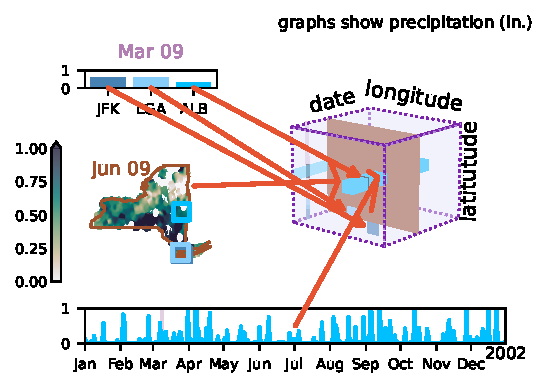
\includegraphics[width=1\columnwidth]{k_different_types.pdf}
  \caption{This weather station data has multiple embedded continuities - points at each time and position, timeseries at each position, and maps at each time. The corresponding visualizations - bar chart, timeseries, and map - each preserve the continuity of the subset of the data they visualize by not introducing or leaving out values and preserving the relative positioning of continuous values.}
%
  \label{fig:related-work:continuity:ktypes}
\end{figure}

Visual algorithms assume the topology of their input data, as described in taxonomies of visualization algorithms Chi\cite{chiTaxonomyVisualizationTechniques2000} and by Troy and M\"{o}ller \cite{toryRethinkingVisualizationHighlevel2004}, but generally do not verify that input structure. For example, a \texttt{line} algorithm often does not have a way to query whether a list of (x,y) coordinates is the distinct rows, the time series, or the list of stations in \autoref{fig:related-work:continuity:ktypes}. While plotting the time series as a continuous line would be correct, it would be incorrect for a visualization to indicate that the distinct rows or stations are connected in a 1D continuous manner because it introduces ambiguity over which part of the line maps back to the data. A map that by definition has continuous maps between the input and output spaces, such as data and graphics, is called a \textit{homeomorphism}\cite{riehlCategoryTheoryContext}:

\begin{definition}
  A function $f$ is a $homeomorphism$ if it is bijective, continuous, and has a continuous inverse function $f^{-1}$.
\end{definition}

The bar plot, line plot, and heatmap in \autoref{fig:related-work:continuity:ktypes} have a homeomorphic relationship to the 0D ($\bullet$) points, 1D (--) linear, and 2D ($\blacksquare$) surface continuities embedded in the continuous 3 dimensional surface encapsulating time and position because each point of the visualization maps back into a point in its corresponding indexing space in the cube. Using homeomorphism to test whether continuity is preserved formalizes Bertin's codification of how the topology of observations matches the class of representation (i.e. point , line, area) \cite{bertinSemiologyGraphicsDiagrams2011} and Wilkinson's assertion that connectivity must be preserved \cite{wilkinsonGrammarGraphics2005}.

To encode topology and field structure in a way that is both uniform and generalizable, we extend Butler's work on using a mathematical structure called fiber bundles as an abstract data representation in visualization \cite{butlerVectorBundleClassesForm1992, butlerVisualizationModelBased1989}. Using this topological model of indexing, semantic indexing as described by Munzner's key-value model of data structure \cite{munznerWhatDataAbstraction2014} act as different ways of partitioning the underlying data continuity. For example, the data cube in \autoref{fig:related-work:continuity:ktypes} could be subset into sets of timeseries where the key would be $station$, or subset into maps where the key would be $date$, or subset into station records where the keys are $(date, latitude, longitude)$. Using a topological model rather than semantic indexing also makes clearer when different labeling schemes refer to the same point, for example how 0-360 and 180E-180W are two ways of labeling longitude or how (date, lat, lon) and (date, station) refer to the same point. We sketch out fiber bundles in \autoref{sec:atct:fiber-bundles}, but Butler provides a thorough introduction to bundles for visualization practitioners.


\subsection{Structure Preservation In Software}
\label{sec:related-work:software}
Visualization libraries are in part measured by how expressive the components of the library are, where expressiveness is a measure of which structure preserving mappings a tool can implement \cite{mackinlayAutomatingDesignGraphical1986}. While some visualization tools aim to automate the pairing of data with structure preserving visual representations, such as Tableau\cite{StoltePolaris2002,hanrahanVizQL2006,MackinlayShowme2007}, many visualization libraries leave that choice to the user. For example, connectivity assumptions tend to be embedded in each of the visual algorithms of `building block` libraries, a term used by Wongsuphasawat \cite{wongsuphasawatNavigatingWideWorld2021,wongsuphasawatNavigatingWideWorld2020} to describe libraries that provide modular components for building elements of a visualization, such as functions for making boxes or translating data values to colors. In building block libraries such as Matplotlib\cite{hunterMatplotlib2DGraphics2007} and D3\cite{bostockDataDrivenDocuments2011} assumptions about connectivity are embedded in the interfaces such that the API is inconsistent across plot types. For example in Matplotlib methods for updating data and parameters for controlling aesthetics differ between (1D) line based plotting methods and (0D) marker based methods. While VTK\cite{hanwellVisualizationToolkitVTK2015,geveciVTK2012} provides a language for expressing the topological properties of the data, and therefore can embed that information in its visual algorithms, VTK's charts API is similar to the continuity dependent APIs of other building block libraries.

Domain specific libraries are designed with the assumption of continuities that are common in the domain \cite{HeerSoftware2006}, and therefore can somewhat restrict their API to choices that are appropriate for that domain. For example, a tabular topological structure of discrete rows, as illustrated in \autoref{fig:related-work:continuity:ktypes}, is assumed by A Presentation Tool\cite{mackinlayAutomatingDesignGraphical1986, mackinlayAutomatingDesignGraphical1986} and grammar of graphics\cite{wilkinsonGrammarGraphics2005} and the ggplot\cite{wickhamGgplot2ElegantGraphics2016}, vega\cite{satyanarayanDeclarativeInteractionDesign2014}, and altair\cite{vanderplasAltairInteractiveStatistical2018} libraries built on these frameworks. Image libraries such as Napari\cite{nicholas_sofroniew_2021_4533308} and ImageJ\cite{schneiderNIHImageImageJ2012} and the ImagePlot\cite{studiesCulturevisImageplot2021} art plugin assume that the input is a 2D continuous image. Networking libraries such as gephi\cite{bastianGephiOpenSource2009} and networkx\cite{HagbergExploringNetwork2008} assume a graph-like structure. By assuming the structure of their data, these domain specific libraries can provide more cohesive interfaces because a limited set of visualization algorithms apply to their data and the visualizations these algorithms provide can be styled in a fixed number of ways.

We propose that the cohesion of domain specific library APIs is obtainable using the uniform data model described in \autoref{sec:atct:fiber-bundles} while the expressivity of building block libraries can be preserved by defining explicit structure preserving constraints on the library components, as described in \autoref{sec:artist}. Because category theory constructions map cleanly to objects and functions, using category theory to express the structure and constraints can lead to more consistent software interfaces in visualization software libraries \cite{wielsManagementEvolvingSpecifications1998,yorgeyMonoidsThemeVariations2012}. A brief visualization oriented introduction to category theory is in Vickers et al \cite{vickersUnderstandingVisualizationFormal2013}, but they are applying category theory to semantic concerns about visualization design rather than library architecture.

\section{Uniform Abstraction for Data \& Graphics}
\label{sec:atct}
In this section, we propose a mathematical abstraction of the data input and pre-rendered graphic output. This mathematical abstraction provides a uniform highly generalizable method for describing topology and fields; expresses how to verify that data continuity is preserved on subset, distributed, and streaming data representations; and formalizes the expectation of a correspondence between data and visual elements. Using these abstractions allows us to embed information about structure in dataset types:

\begin{equation*}
  \textcolor{section}{\texttt{dataset}}: \textcolor{base}{\texttt{topology}} \rightarrow \textcolor{fiber}{\texttt{fields}}
\end{equation*}

which can then be checked by visualization algorithms to ensure that the assumptions of the data match the assumptions of the algorithm. This typing system also extends to pre-rendered graphic output, allowing us to develop the structure preservation framework in \autoref{sec:artist} that ensures that output fields are equivalent to the input fields and that the topology of the output graphic is homeomorphic to the topology of the input.

\subsection{Abstract Data Representation}
\label{sec:atct:fiber-bundles}
We model data using a mathematical representation of data that can encode topological properties, field types, and data values in a uniform manner using a structure from algebraic topology called a fiber bundle. We extend Butler's proposal of using bundles as an abstraction for visualization data\cite{butlerVectorBundleClassesForm1992,butlerVisualizationModelBased1989} by incorporating Spivak's methodology for encoding named data types from his fiber bundle representation of relational databases \cite{spivakDatabasesAreCategories2010,spivakSimplicialDatabases2009}. We build on this work to describe how to encode the connectivity of the data as a topological \textcolor{base}{base space} modeling the data indexing space, encode the fields as a \textcolor{fiber}{fiber space} that acts as the data schema (domain), and express the mappings between these two spaces as \textcolor{section}{section} functions that encode datasets as mappings from indexing space to field space \texttt{dataset: topology $\rightarrow$ fields}.

\begin{definition}\label{def:fiber_bundle}
   A \textbf{fiber bundle} $(\dtotalc, \dbasec, \pi, \dfiberc)$ is a structure with topological spaces $\dtotalc, \dfiberc, \dbasec$ and  bundle projection map $\pi: \dtotalc \rightarrow \dbasec$ \cite{spanier1989algebraic}.

   \begin{equation} \label{eq:atct:fb:intro}
    \begin{tikzcd}
      \dfiberc \arrow[r, hook, color=total] & \dtotalc \arrow[r, "\pi", color=total, two heads] & \dbasec
      \end{tikzcd}
    \end{equation}

A continuous surjective map $\bm{\pi}$ is a \textbf{bundle projection} map when
\begin{enumerate}
  \item all fibers in the bundle are isomorphic. Since all fibers are isomorphic $\dfiber \cong \dfiber_{\dbasepoint}$ for all points $\dbasepoint \in \dbase$, there is a uniquely determined \textcolor{fiber}{fiber space} \dfiberc\ given by the preimage of the projection $\pi$ at any point $\dbasepoint$ in the \textcolor{base}{base space} \dbasec: $\dfiberc = \pi^{-1}(k)$.
  \item each point $\dbasepointc$ in the \textcolor{base}{base space} \dbasec\ has an open neighborhood $\openset_{\dbasepointc}$ such that the \textcolor{total}{total space} \dtotalc\ over the neighborhood is locally trivial.
\end{enumerate}
\end{definition}

\textbf{Local triviality} means $\dtotal\vert_{\openset} = \openset\times \dfiber$. In this paper we use $\dtotal\vert_{\openset} = \pi^{-1}(\openset)$ to denote the preimage of an openset\footnote{Open sets (open subsets) are a generalization of open intervals to n dimensional spaces. For example, an open ball is the set of points inside the ball and excludes points on the surface of the ball. \cite{weissteinOpenSet,bradleyTopologyVsTopology}}, and a \textbf{local trivialization} is a specific choice of neighborhoods (described in \autoref{sec:atct:fb:base}) and their preimages such that the fibers in each preimage are identical $\dfiber = \dfiber_{\dbasepoint}$ for all points $\dbasepoint \in \openset$. All fiber bundles can be decomposed into sets of local trivializations that are also bundles and we can specify a gluing scheme that reconstructs the fiber bundle from locally trivial pieces by specifying\textbf{transition maps} for all overlaps of the local trivializations; therefore, while the framework in this paper applies to all bundles, in this paper we assume that the bundles are trivial bundles $\dtotal = \dbase \times \dfiber$ so that we can assign all fibers in a bundle the same type. For an example of trivial and non-trivial bundles, see \autoref{sec:appendix:bundle_triviality}.

\begin{minipage}{.5\columnwidth}
\begin{definition}\label{def:fiber_bundle:section}
A \textcolor{section}{\textbf{section}} $\dsectionc: \dbasec \rightarrow \dtotalc$ over a fiber bundle is a smooth right inverse of $\pi(\dsection(\dbasepoint)) = \dbasepoint$ for all $\dbasepoint \in \dbase$
\end{definition}
\end{minipage}
\begin{minipage}{.4\columnwidth}
  \begin{equation} \label{eq:atct:fb:intro-sec}
    \begin{tikzcd}[ampersand replacement=\&, row sep=huge]
     \dfiberc
      \arrow[r, hook, color=total] \&
      \dtotalc
      \arrow[d, "\pi"',color=total, two heads] \\
       \&
    \dbasec
       \arrow[u, "\dsectionc"', bend right, pos=.5, color=section, dashed]
    \end{tikzcd}
  \end{equation}
\end{minipage}

We propose that the total space of a bundle can encode the mathematical space in which a  dataset is embedded, the base space can encode the topological properties of the dataset, the fiber space can encode the data types of the fields of the dataset, and that the datasets can be encoded as section functions from the continuity to the fiber space.

\begin{figure}[!h]
       \includegraphics[width=1\columnwidth]{fb.pdf}
       \caption{The space of all data values encoded by this fiber bundle can be modeled as a \textcolor{total}{rectangle} total space. Each dataset in this data space lies along the interval \textcolor{base}{$[0,2\pi]$} base space. Each dataset has values along the \textcolor{fiber}{$-1 \rightarrow 1$} interval fiber. One dataset embedded in this total space is the \textcolor{section}{sin} section over the bundle.}\label{fig:atct:fb}
  \end{figure}


For example, the fiber bundle in \autoref{fig:atct:fb} encodes the space of all continuous functions that have a domain of $[0, 2\pi]$ and range $[0,1]$. Using a fiber bundle abstraction encodes that the dataset has a 1D linear continuity as the base space \dbase is the interval $[0,2\pi]$ and a field type that is a \texttt{float} in the range $[0,1]$. Therefore the type signature of the datasets in this fiber bundle, which is called a section \dsection, would be \texttt{dataset: $[0, 2\pi] \rightarrow [0,1]$}. One such dataset (section) is the $\sin$ function, which as shown in \autoref{fig:atct:fb} is defined via a function \dsection from a point in the base space to a corresponding point in the fiber. Evaluating the section function over the entire base space yields the $\sin$ curve that is composed of points intersecting each fiber over the corresponding point. The local trivializations shown in \autoref{fig:atct:fb} are one way of decomposing the total bundle and conversely the bundle can be constructed from the local trivializations $\dbase = \dbase_{0} \oplus \dbase_{1}$. As shown, the section $\sin$ spans the trivializations in the same manner that it spans the bundle; this is analogous to how a dataset may span multiple tables or be collected in one table. The trivializations are glued together into the bundle at the overlapping region $\frac{2\pi}{5}$ by defining the transition map $\dfiber_{1} \rightarrow \dfiber_{2}$. Because the fibers in \autoref{fig:atct:fb} at $\frac{2\pi}{5}$ are aligned, the transition map is an identity map that take every value in $\dfiber_1$ and maps it to the same value in $\dfiber_2$ so that the sections, such as $\sin$, remain continuous.


\subsubsection{\textcolor{base}{Topological Structure: Base Space \dbase}}
\label{sec:atct:fb:base}

We encode the topological structure of the data as the \textcolor{base}{base space} of a fiber bundle. Describing connectivity using the language of topology allows for describing individual elements in a way that holds true whether the data fits in memory, is distributed, or is streaming. This is because, informally, a topology $\mathcal{T}$ on the underlying data indexing space (which is a proxy for the continuity), is a partitioning of that space such that the partitions are of the same mathematical type as each other and the partitioned space. The partitions must also be composable in a continuity and property preserving way.

There are various equivalent definitions of topology, but here we use the neighborhood axiomatization because it is most analogous to the data access model of index (element) in subset (neighborhood) of all indices (mathematical space). Given a set $X$ and a function $\mathcal{N}:X\to 2^{2^X}$ that assigns to any $x\in X$ a non-empty collection of subsets $\mathcal{N}(x)$, where each element of $\mathcal{N}(x)$ is a \emph{neighborhood of $x$}, then $X$ with  $\mathcal{N}$ is a \textcolor{base}{topological space} and $\mathcal{N}$ is a neighborhood \emph{topology} if for each $x$ in $X$: \cite{brownronaldTopologyGroupoids2006}

\begin{definition}\label{def:topology}
\begin{enumerate}
  \item if $N$ is a neighborhood $N \in \mathcal{N}(x)$ of $x$ then $x \in N$
  \item every superset of a neighborhood of $x$ is a neighborhood of $x$; therefore a union of a neighborhood and adjacent points in $X$ is also a neighborhood of $x$
  \item the intersection of any two neighborhoods of $x$ is a neighborhood of $x$
  \item any neighborhood $N$ of $x$ contains a neighborhood $M \subset N$ of $x$ such that $N$ is a neighborhood of each of the points in $M$
\end{enumerate}
\end{definition}

Therefore a neighborhood has to contain $x$ (1), can grow (2), or shrink (3), and every neighborhood also contains smaller neighborhoods of points adjacent to x (4). For example, in the indexing cube in \autoref{fig:fig:related-work:continuity:ktypes}, the brown surface and blue rectangle are both neighborhoods of the index for the measurement in Albany on June 09. The blue rectangle is also a neighborhood of the index for the measurement in Albany on March 09. The indexing cube is a neighborhood for both of these indices. While \autoref{def:topology} applies broadly to topological spaces, in this paper we usually model the indexing space as CW-complexes. CW-complexes are a class of topological spaces built by gluing together n-dimensional balls (which include points, intervals, filled circles, filled spheres, etc.) using continuous attaching maps. Because the base space of a fiber bundle is a quotient topology\cite{munkresElementsAlgebraicTopology1984}, it divides the topological space into the largest number of open sets such that $\pi$ remains a continuous function. This means that the topology can be defined to have a resolution equal to the number of indices in a dataset such that the key (continuity)-value (data) pairing is always preserved.

Following from Spivak's categorical abstraction of a database \cite{spivakSimplicialDatabases2009,spivakDatabasesAreCategories2010}, we also propose that the structure of the data types be formally specified as the objects of a category.

\begin{definition}\label{def:atct:category}
   An \textbf{category} $\mathcal{C}$ consists of the following \textit{data}:
\begin{enumerate}
  \item a collection of \textit{objects} $X \in \textbf{ob}(\mathcal{C})$
  \item for every pair of objects $X, Y \in \textbf{ob}(\mathcal{C})$, a set of \textit{morphisms} $X \xrightarrow{f} Y \in Hom_{\mathcal{C}}(X, Y)$
  \item for every object $X$, a distinct \textit{identity morphism} $X \xrightarrow {id_x} X$ in $Hom_{\mathcal{C}}(X, X)$
  \item a \textit{composition function} $f \in Hom_{\mathcal{C}}(X, Y) \times  g \in Hom_{\mathcal{C}}(Y, Z) \rightarrow g \circ f \in Hom_{\mathcal{C}}(X, Z)$
\end{enumerate}
such that
\begin{enumerate}
  \item \textit{unitality:} for every morphism $ X \xrightarrow{f} Y$, $f \circ id_x = f = id_y \circ f$
  \item \textit{associativity:} if any three morphisms $f, g, h$ are composable,
    \begin{equation*}
      \begin{tikzcd}
        X \arrow[r, "f"] \arrow[rrr, "h\circ(g\circ f) = (h\circ g)\circ f"', bend right, dashed] & Y  \arrow[r, "g"] & Z \arrow[r, "h"] & W
        \end{tikzcd}
  \end{equation*}
  then they are associative such that $h\circ(g\circ f) = (h \circ g) \circ f$  \cite{lawvere2009conceptual,riehlCategoryTheoryContext,maclaneCategoriesWorkingMathematician2013,fongInvitationAppliedCategory2019}.
  \end{enumerate}
\end{definition}

The standard construction of a category from a topological space is that it has open set objects $\opensetc$ and inclusion morphisms $\opensetc_i \xrightarrow{\iota} \opensetc_j$ such that $\opensetc_i \subseteq \opensetc_j$\cite{riehlCategoryTheoryContext}. The composability property expresses that inclusion is transitive, while associativity expresses that the inclusion functions can be curried in various equivalent groupings. By formally specifying the properties of the topological structure data types as $\mathcal{\dbase}$, we can express that these are the properties that are required as part of the implementation of the data type objects.

\paragraph{Joining indexing spaces: $\oplus: \mathcal{\dbasec} \sqcup \mathcal{\dbasec} \rightarrow \mathcal{\dbasec}$}
Joining two bundles on their base space, for example to glue the two trivializations in \autoref{fig:atct:fb} into a bundle, is the coproduct $\dbase_{a} \sqcup_{\dbase_{c}} \dbase_{b}$ over a space $\dbase_{c}$. A property of the coproduct is that the inclusion morphism must be commutative, which means that index spaces are combined on overlapping indices:
\begin{figure}[h]
  \includegraphics*[width=1\columnwidth]{figures/tex/k_coproduct.pdf}  \caption{Index spaces are combined via the \textit{coproduct} $\dbase_{a}\sqcup_{\dbase_c} \dbase_{b}$.}
  \label{fig:atct:base}
\end{figure}
 For example, in \autoref{fig:atct:base}, the open interval $\dbase_c$ is present in both $\dbase_a$ and $\dbase_c$; therefore $\dbase_a$ and $\dbase_b$ are glued together where they overlap at $\dbase_c$.  Two spaces have been combined correctly if every point in the overlap  $\dbasepoint \in \dbase^{c}$ is present in each of the spaces $\dbasepoint \in \dbase^{a}$ and $\dbasepoint \in \dbase^{b}$ such that it is present in the joined space $\dbasepoint \in \dbase^{a}\sqcup_{\dbase^{c}} \dbase_{b}$. This simple test that the records are joined correctly is what allows us to reliably build larger datasets out of smaller ones, such as in the case of distributed and on demand datasets.


\subsubsection{\textcolor{fiber}{Data Field Types: Fiber Space \dfiber}}
\label{sec:atct:fb:fiber}
As mentioned in \autoref{sec:related-work:equivariance}, visualization researchers traditionally describe equivariance as the preservation of field structure, which is based on the field type. Spivak shows that data typing can be expressed in a categorical framework in his fiber bundle formulation of tables in relational databases \cite{spivakDatabasesAreCategories2010,spivakSimplicialDatabases2009}. In this work, we adopt Spivak's definitions of \textit{type specification}, \textit{schema}, and \textit{record} because that allows us to use a dimension agnostic named typing system for the fields of our dataset that is consistent with the abstraction we are using to express the continuity. Spivak introduces a \textit{type specification} as a bundle map $\pi: \mathscr{U} \rightarrow \textbf{DT}$. The base space $\textbf{DT}$ is a set of data types $T \in \textbf{DT}$ and the total space $\mathscr{U}$ is the disjoint union of the domains of each type \[\mathscr{U} = \bigsqcup_{T \in \textbf{DT}} \pi^{-1}(T)\] such that each element $x$ in the domain $\pi^{-1}(T)$ is one possible value of an object of type $T$ \cite{spivakSimplicialDatabases2009}. For example, if $T=\texttt{int}$, then the image $\pi^{-1}(\texttt{int}) = \mathbb{Z} \subset \mathscr{U}$ is the set of all integers and $x=3 \in \mathbb{Z}$ is the value of one $\texttt{int}$ object.

Since many fields can have the same datatype, Spivak formally defines a mapping from field name to field data type, akin to a database schema \cite{ullmanFirstCourseDatabase2008}. According to Spivak, a \textit{schema} consists of a pair $(\fnames, \sigma)$ where $\fnames$ is the set of field names and $\sigma: \fnames \rightarrow \textbf{DT}$ is a function from field name to field data type\cite{spivakSimplicialDatabases2009}. The function $\sigma$ is composed with $\pi$ such that $\pi^{-1}(\sigma(C)) \subseteq \mathscr{U}$; this composition induces a domain bundle $\pi_{\sigma}:\mathscr{U}_{\sigma} \rightarrow \fnames$ that associates a field name $c \in C$ with its corresponding domain $\pi^{-1}_{\sigma}(C) \subseteq \mathscr{U}_{\sigma}$.
\begin{definition} A \textbf{record} is a function $\delement: \fnames \rightarrow \mathscr{U}_{\sigma}$ and the set of records on $\pi_{\sigma}$ is denoted $\Gamma^{\pi}(\sigma)$. Records must return an object of type $\sigma(\fname) \in \textbf{DT}$ for each field $c \in C$.
\end{definition}
Spivak then describes tables as sections $\dsection: \dbase \rightarrow \Gamma^{\pi}(\sigma)$ from an indexing space $\dbase$ to the set of all possible records $\Gamma^{\pi}(\sigma)$ on the schema bundle, and his notion of a table generalizes to our notion of a data container.

To build on the rich typing system provided by Spivak, we define the \textcolor{fiber}{fiber space} \dfiberc\ to be the space of all possible data records
\begin{equation}
  \dfiberc \coloneqq \{\delement: \fnames \rightarrow \mathscr{U}_{\sigma} \bigm{\vert} \pi_{\sigma}(\delement(\fname)) = \fname\;for\;all\; \fname \in \fnames \}
\end{equation}
such that the preimage of a point is the corresponding data type domain $\pi^{-1}(\dbasepoint) = \dfiber_{k} = \mathscr{U}_{{\sigma}_{\dbasepoint}}$.
Adopting Spivak's fiber bundle construction of types allows our model to reuse types so long as the field names are distinct and that field values can be accessed by field name,  since those are sections on $\mathcal{U}_{\sigma}$. Furthermore, since domains $\mathscr{U}_{{\sigma}}$ of types are a mathematical space, multi-dimensional fields can be encoded in the same manner as single dimensional fields and fields can have different names but the same type.

As with the base space category $\mathcal{\dbase}$, we propose a fiber category $\mathcal{\dfiberc}$ to encapsulate the field types of the data. The fiber category has a single object $\dfiberc$ of an arbitrary type and morphisms on the fiber object $\dfunctc \in Hom(\dfiberc, \dfiberc)$. We can also equip the category with any operators or relations that are part of he mathematical structure of the field type. For example we can equip the category with a comparison operator, which is part of the definition of the monoidal structure of a partially ordered ranking variable \cite{bruggemannRankingPrioritizationMultiindicator2011} or the group structure of Steven's ordinal measurement scale \cite{stevensTheoryScalesMeasurement1946, leaFormalizationMeasurementScale1971, thomasMathematizationNotMeasurement2014}. Steven's other scales are summarized in \autoref{tab:appendix:summary:stevens}.

\paragraph{Merging fields: $\otimes: \mathcal{\dfiber} \times \mathcal{\dfiber} \rightarrow \mathcal{\dfiber}$ }

The fiber category $\mathcal{\dfiberc}$ is also equipped with a bifunctor because it is a monoidal category and this functor provides a method for combining fiber types. The bifunctor allows $\otimes$ us to express fields that contain complexly typed values. For example, dates can be represented as three fields $\dfiber_{year} \times \dfiber_{month} \times \dfiber_{day}$ or a composite fiber field $\dfiber_{year} \times \dfiber_{month} \times \dfiber_{day} = \dfiber_{date}$. The $\otimes$ encapsulates both the sets of values associated with each fiber $\{y \in \mathbb{I}\vert 1992 \leq y \leq 2025\} \times \{m \in \mathbb{I}\vert 1 \leq m \leq 12 \} \times \{d \in \mathbb{I}\vert 1 \leq d \leq 31 \}$ and the composition function $ \otimes: \dfiber_{year} \times \dfiber_{month} \times \dfiber_{day} \rightarrow \dfiber_{date}$
would include a constraint to only return dates that have the right number of days for each month. The bifunctor also composes the morphisms associated with each category into a morphism on the composite category $(\dfunct_{year}, \dfunct_{month}, \dfunct_{day}) = \dfunct_{date}$.

Combining fibers correctly can be verified by checking that when a fiber component $\dfiber^{c}$ is present in both $\dfiber^{a}$ and $\dfiber^{b}$, it is identical when projected out of either such that the \textit{product} diagram commutes, means that when data with many fields is decomposed into its component fields, records maintain their integrity:

\begin{figure}[H]
  \includegraphics*[width=1\columnwidth]{figures/tex/f_product.pdf}
  \caption{Fields are combined via the \textit{product} $\dfiber_{a}\times_{\dfiber_c} \dfiber_{b}$.}
  \label{fig:atct:fiber}
\end{figure}

For example in \autoref{fig:atct:fiber} the red (temperature, time, pressure) record separates into (temperature, time) and (pressure, time) records that share the same red time. Furthermore this time is the same whether it is obtained from the (temperature, time) or (pressure, time) record. Generally, the test for joining fields is that when a record is present in a fiber $\delement_{c} \in \pi_c(\dfiber_{a}), \delement_c \in \pi_c(\dfiber_{b})$ then it is in the joint record $\delement_{c} \in \pi_c(\dfiber_{a}\times_{\dfiber_c}\dfiber_{b})$ when is in the field $\dfiber_c$ being joined on. This simple test that fields are joined together correctly for the same record is what allows us to reliably combine multiple datasets together on shared properties, for example growing the weather station data in \autoref{fig:related-work:continuity:ktypes} from a temporal to spatial dataset by adding the weather at each location at each time.

\subsubsection{\textcolor{section}{Data: Section $\dsection$}}
\label{sec:atct:fb:sections}
We encode data as a \textcolor{section}{section} \dsectionc\ of a bundle because this allows us to incorporate the topology and field types in the data definition. We define section functions locally, meaning that the section is (piece-wise) continuous over a specific open subset \openset\ of \dbase\:
\begin{equation}
  \label{eq:atct:fb:sections}
  \cgamma{\opensetc}{\dtotalc\restriction_{\opensetc}} \coloneqq \big\{\dsectionc: \opensetc\rightarrow \dtotalc\restriction_{\opensetc} \; \bigm{\vert} \pi(\dsectionc(\dbasepointc)) = \dbasepointc\;for\, all\; \dbasepointc \in \opensetc \big\}
\end{equation}
such that each section function $\dsection: \dbasepoint \mapsto \delement$ maps from each point $\dbasepoint \in \openset$ to a corresponding record in the fiber space $\delement \in \dfiber_{\dbasepoint}$ over that point. Bundles can have multiple sections, as denoted by $\Gamma(\openset, \dtotal\restriction{\openset})$. We can therefore model data as structures that map from an index like point $\dbasepoint$ to a data record $\delement$, and encapsulate multiple datasets with the same fiber and base space as different sections of the same bundle.

When a bundle is trivial $\dtotalc = \dbasec \times \dfiberc$, we can defined a global sections $\dsection: \dbase \rightarrow \dfiber \in \Gamma(\dbase, \dfiber)$ which we translate into a data signature of the form $\textcolor{section}{\texttt{dataset}}: \textcolor{base}{\texttt{topology}} \rightarrow \textcolor{fiber}{\texttt{field}}$ where $\dsectionc=\textcolor{section}{\texttt{dataset}}$, $\dbasec=\textcolor{base}{\texttt{topology}}$ and $\dfiberc=\textcolor{fiber}{\texttt{fields}}$. When the bundle is non-trivial, we can use the fiber bundle property of local-triviality to define local sections $\dsection\restriction_{\openset} \in \Gamma(\openset_{\dbasepoint}, \dtotal\restriction_{\openset_{\dbasepoint}})$. A local section is defined over an open neighborhood  $\dbasepoint \in \openset \in \dbase$, which is an open set that surrounds a point \dbasepoint. Most data sets can be encoded as a collection of local sections $\{\dsection\restriction_{\openset_{\dbasepoint}}| \dbasepoint \in \dbase \}$ and this encoding can be translated into a set of signatures $\{\textcolor{section}{\texttt{data-subset}}: \textcolor{base}{\texttt{topology}} \rightarrow \textcolor{fiber}{\texttt{fields}}$ s.t. $\textcolor{section}{\texttt{data-subset}} \subset \textcolor{section}{\texttt{dataset}}\}$. The subsets of the fiber bundle and the transition maps between these subsets are encoded in an atlas\cite{ghristElementaryAppliedTopology2014} and the notion of an atlas can be incorporated into the data container, as discussed in \autoref{sec:atct:sheaves}.

\subsubsection{Example: Uniform Abstract Graphic Representation}
One of the reasons we use fiber bundles as an abstraction is that they are general enough that we can also encode the output of a visual algorithm as a bundle. We denote the output as a graphic, but the use of bundles allows us to generalize to output on any display space, such as a screen or 3D print.
\begin{equation}
  \label{eq:atct:fb:graphic}
  \begin{tikzcd}
      \gfiberc \arrow[r, hook, color=total] & \gtotalc \arrow[r, "\pi", two heads, color=total] & \gbasec
  \end{tikzcd}
\end{equation}
The total space \gtotalc\ is an abstraction of an ideal (infinite resolution) space into which the graphic can be rendered. The base space \gbasec\ is a parameterization of the display area, for example the inked bounding box in the cairo \cite{CairographicsOrg} rendering library. The fiber space \gfiberc\ is an abstraction of the renderer fields; for example a 2 dimension screen has pixels that can be parameterized $ \gfiber=\{x,\,y\,z,\,r,\,g,\,b,\,a\}$. As with data, we model the graphic specifications as sections $\gsection$ of the graphic bundle
\begin{equation}\label{eq:atct:fb_graphic_section}
  \begin{split}
  \cgamma{\opensetgc}{\gtotalc\restriction_{\opensetgc}} & \coloneqq \\
  &\big\{\gsectionc: \opensetgc\rightarrow \gtotalc\restriction_{\opensetgc} \; \bigm{\vert} \pi(\gsectionc(\gbasepointc)) = \gbasepointc\;for\, all\; \gbasepointc \in \opensetgc \big\}
  \end{split}
\end{equation}
that map from a point in an openset in the graphic space $\gbasepoint \in \opensetg \subseteq \gbase$ to a point in the graphic fiber $\gfiber$. The section evaluated on a single point $\gbasepoint$ returns a single graphic record, for example one pixel in an ideal resolution space. In our model, the unevaluated graphic section is passed from the visualization library component to the renderer to generate graphics.

\begin{figure}[]
  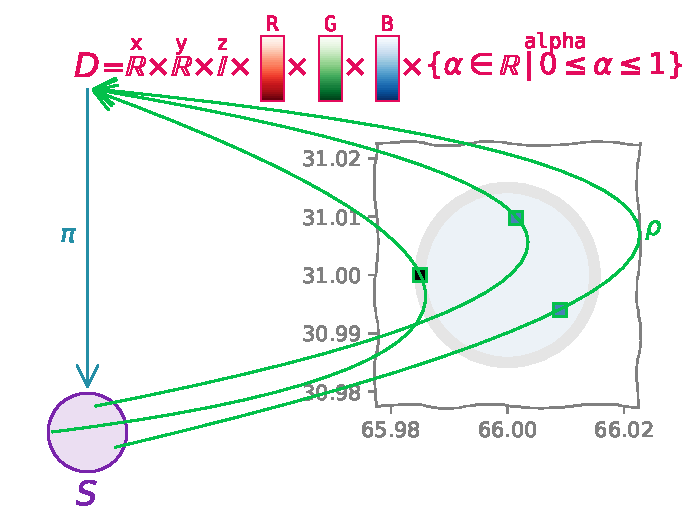
\includegraphics[width=1\columnwidth]{fb_rho.pdf}
  \caption{The scatter marker is specified by the section $\gsection$, which maps into the fiber $\gfiber$ to retrieve the values that compose into the pixel (approximated as a square) returned by the section function evaluated at each point $\gbasepoint$. The section evaluated over the entire space $\gsection\vert_{S}$ returns the entire scatter mark, shown here in faded form to make it easier to see the individual pixels.
  \label{fig:atct:fb:graphic}}
\end{figure}

In \autoref{fig:atct:fb:graphic}, the section function $\gsection$ maps into the fiber for a simplified 2D RGB infinite resolution pre-render space and returns the $\{x,y,r,g,b\}$ values of a pixel in an infinite resolution space. In \autoref{fig:atct:fb:graphic} these pixels are approximated as the small colored boxes. Each pixel is the output of the $\gsection(\gbasepoint)$ section that intersects the box. The set of all pixels returned by a section evaluated on a given visual base space $\gsection|_{\gbase}$ can yield a visual element, such as a marker, line, or piece of a glyph and in $\autoref{fig:atct:fb:graphic}$ is a blue circle with a black edge. While \autoref{fig:atct:fb:graphic} illustrates a highly idealized space with no overlaps, overlaps can be managed via a fiber element $\gfiber_{z}$ for ordering. It is left to the renderer to choose how to blend $\gfiber_{z}$ and $\gfiber_{a}$ layers.

\subsection{Abstract Data Containers}
\label{sec:atct:sheaves}
While bundles provide a way to describe the structure of the data, sheaves are a mathematical way of describing the data container. Sheaves are an algebraic data structure that provides a way of abstractly discussing the bookkeeping that data containers must implement to keep track of the continuity of the data \cite{ghristElementaryAppliedTopology2014}. This abstraction facilitates representational invariance, as introduced by Kindlemann and Scheidegger\cite{kindlmannAlgebraicProcessVisualization2014}, since the container level is uniformly specified as satisfying presheaf and sheaf constraints. When a data container satisfies these constraints, the subsets and whole data space have the same mathematical properties, e.g. morphisms, such that the framework in this paper applies whether the data is in memory, distributed, streaming, or on-demand.

We can mathematically encode that we expect data containers to preserve the underlying continuity of the indexing space and the mappings between indexing space and record space using a type of function called a functor. Functors are mappings between categories that preserve the domains, codomains, composition, and identities of the morphisms within the category\cite{riehlCategoryTheoryContext}.

\begin{definition}\cite{bradleyWhatFunctorDefinitions,bradleyTopologyCategoricalApproach2020} A \textbf{functor} is a map $F: \mathcal{C} \rightarrow \mathcal{D}$, which means it is a function between objects $F: \textbf{ob}(\mathcal{C}) \mapsto \textbf{ob}(\mathcal{D})$ and that for every morphism $f \in Hom(C_1, C_2)$  there is a corresponding function $F: Hom(C1, C2) \mapsto Hom(F(C_1), F( C_2))$.
A \textbf{functor} must satisfy the properties
\begin{itemize}
  \item \textit{identity}: $F(id_{C}(C)) = id_{D}(F(C))$
  \item \textit{composition}: $F(g)\circ F(f) = F(g\circ f)$ for any composable morphisms $C_{1}\xrightarrow{f} C_2$, $C_2 \xrightarrow{g} C_3$
\end{itemize}
$F(C) \in \textbf{ob}(\mathcal{D})$ denotes the object to which an object $C$ is mapped, and $F(f) \in Hom(F_(C_1), F_(C_2))$ denotes the morphism that $f$ is mapped to.
\end{definition}
Modeling the data container as a functor allows us state that, just like a functor, the container is a map between index space objects and sets of data records that preserve morphisms between index space objects and data records.
\begin{equation}
  \label{eq:atct:sheaf:functor}
  \sheafc_{\dbasec, \dtotalc}: \opensetc \rightarrow \cgamma{\opensetc}{\dtotalc\restriction_{\opensetc}}
\end{equation}
A common way of encapsulating a map from a topological space to a category of sets is as a presheaf
\begin{definition}\label{def:atct:presheaf}
  A \textbf{presheaf} $F:\mathcal{C}^{op} \rightarrow \setb$ is a contravariant functor from an object in an arbitrary category to an object in the category \setb\cite{spanier1989algebraic}.
\end{definition}

A functor is contravariant when the morphisms between the input objects go in the opposite direction from the morphisms between the output objects. The presheaf is contravariant when for every arbitrary morphism between input base spaces $\dfunch: \openset_1 \rightarrow \openset_2$ there exists a corresponding pullback function between the sets of sections $\dfuncpull: \cgamma{\opensetc_2}{\dtotalc\restriction_{\opensetc_2}} \rightarrow \cgamma{\opensetc_1}{\dtotalc\restriction_{\openset_c1}}$.


%% these two paragraphs cen be condensed and moved below the figure as an example
A functor is contravariant when the morphisms between the input objects go in the opposite direction from the morphisms between the output objects. The presheaf is contravariant because the inclusion morphisms between input object $\iota: \opensetc_1 \rightarrow \opensetc_2$
are defined such that they correspond to the partial ordering $\openset_1 \subseteq \openset_2$, but the restriction morphisms $\iota^*$ between the sets of sections $\iota^*: \cgamma{\opensetc_2}{\dtotalc\restriction_{\opensetc_2}} \rightarrow \cgamma{\opensetc_1}{\dtotalc\restriction_{\openset_c1}}$ restricts the larger set to the smaller one such that all functions that are continuous over a space must be continuous over a subspace $\Gamma_2 \subseteq \Gamma_1$, where $\Gamma_{i}\coloneqq\Gamma(\openset_{i}, \dtotal\restriction_{\openset_{i}})$.

Data containers that implement managing subsets in a structure preserving way are satisfying the  presheaf constraints that subsets of the indexing space $\openset_1$ are included in any index $\openset_2$ that is a superset $\iota$ and that data defined over an indexing space must exist over any indexes inside that space $\iota^*$. For example, lets define presheaves $\sheaf_1, \sheaf_2$. These are maps from intervals $\openset_1, \openset_2$ to a set of functions $\Gamma_1, \Gamma_2$ that are continuous over that interval:

\begin{figure}[H]
  \includegraphics*[width=1\columnwidth]{figures/tex/presheaf.pdf}
  \caption{Modeling this data container as a presheaf specifies that since $\cos, \sin, and \texttt{C}$ are continuous over $\openset_{2}$, they must be continuous over $\openset_{1}$ since $\openset_1$ is a subset of and therefore must be included in $\openset_2$. Because $\tan$ is only defined over $\openset_{2}$, it does not need to be included in the set $\Gamma_{2}$. \label{fig:atct:presheaf}}
\end{figure}

For example in \autoref{fig:atct:presheaf}, since the $constant, sin, cos$ functions are defined over the interval $\left[0,2\pi\right]$, these functions must also be continuous over the sub-interval $\left(\frac{\pi}{2}, \frac{3\pi}{2}\right)$; therefore the sections in $\Gamma_{2}$ must also be included in the set of sections over the subspace $\Gamma_{1}$. One generalization of this constraint is that data structures that contain continuous functions must support interpolating them over arbitrarily small subspaces.

While presheaves preserve the rules for sets of sections, sheaves add on conditions for gluing individual sections over subspaces into cohesive sections over the whole space.These are the conditions that when satisfied ensure that a data container is managing distributed and streaming data in a structure preserving way.

\begin{definition}\label{def:atct:sheaf}\cite{bakerEuclideanSpaceMathsSheaf,spanier1989algebraic} A \textbf{sheaf} is a presheaf that satisfies the following two axioms
\begin{itemize}
  \item \textit{locality} two sections in a sheaf are equal $\dsection^{a} = \dsection^{b}$ when they evaluate to the same values $\dsection^{a}\vert_{\openset_i} =  \dsection^{b}\vert_{\openset_i}$ over the open cover $\bigcup_{i\in I} \openset_{i} \subset \openset$ (indexed by $I$).
  \item \textit{gluing} the union of sections defined over subspaces $\dsection^{i} \in \Gamma(\openset_i, \dtotal|_{\openset_i})$ is equivalent to a section defined over the whole space $\dsection\vert_{\openset_i} = \dsection^{i}$ for all $i\in I$ if all pairs of sections agree on overlaps $\dsection^{i}\vert_{\openset_i\cap\openset_j} =  \dsection^{j}\vert_{\openset_i\cap\openset_j}$
  \end{itemize}
\end{definition}

The gluing axiom says that a distributed representation of a dataset, which is a set of local sections, is equivalent to a section over the union of the opensets of the local sections. The gluing axiom can also be used to generate the gluing rules used to construct non-trivial bundles from the set of trivial local sections. The locality axiom asserts that the glued section function is equivalent to a function over the union if they evaluate to the same values.

\begin{figure}[h]
  \includegraphics[width=1\columnwidth]{tex/sheaf_rules.pdf}
  \caption{A sheaf has the conditions that sections are equal when they match on all subsets (\textit{locality}) and that the sections can be concatenated when they match on overlaps \textit{gluing}.\label{fig:atct:sheaf}}
\end{figure}

For example, in \autoref{fig:atct:sheaf}, the $\tau^{a}$ and $\tau^{b}$ $\sin$ sections are equal because they match \textit{locally} on all subsets. This is true whether $\sin$ is defined over parts ($\sin\vert_{\openset_i}$) or the whole space. If $\sin$ is defined over parts, then those parts can be \textit{glued} together. The concatenated $\sin$ is continuous because the pieces of the section outside the overlap are continuous with the pieces inside the overlap. The glued $\sin$ is also equal to the non-glued $\sin$ because they match on the opensets; therefore they are equivalent representations of the same section $\sin$ and so have the same mathematical properties.

While each section of a sheaf is evaluated over a point $\dsection(\dbasepoint)$ such that it returns a single record, the sheaf model also provides an abstraction when neighboring information is required. The sheaf over a very small region surrounding a point $\dbasepoint$ is called a \textit{stalk}\cite{harder2008lectures}
\begin{equation}
  \label{eq:atct:sheaf:stalk}
    \sheaf_{\dbase, \dtotalc}\restriction_{\dbasepoint}\coloneqq \lim\limits_{\openset\ni \dbasepoint} \Gamma(\openset, \dtotal\restriction_{\openset})
\end{equation}
where the fiber is contained inside the stalk  $\dfiber_{\dbasepoint} \subset  \sheaf_{\dbase, \dtotal}\restriction_{\dbasepoint}$. The \textit{germ} is the section evaluated at a point in the stalk  $\dsection(\dbasepoint) \in \sheaf_{\dbase, \dtotal}\restriction_{\dbasepoint}$ and is the data. Since the stalk includes the values near the limit of the point at \dbasepoint\, the germ can be used to compute the mathematical derivative of the data for visualization tasks that require this information.

\subsection{Data Index and Graphic Index Correspondence}
\label{sec:atct:xi}
When data and graphic containers are modeled as sheaves and there is a continuous map between their base spaces, the properties of sheaves can be used to describe how visual elements correspond to distinct data elements, which is a necessary condition of a visualization being readable\cite{ziemkiewiczEmbeddingInformationVisualization2009}. We propose that if a visualization is structure preserving, there exists a homeomorphic map \vindexc\ between the graphic indexing space \gbase\ and the data indexing space \dbase\ that maps multiple graphic indexes to one data index such that every index in the graphic space can be mapped to an index in the data space. We define the mapping \vindexc\ to be a surjective continuous map:
\begin{equation}
  \label{eq:atct:xi}
  \vindexc: \opensetgc \textcolor{functor}{\rightarrow} \opensetc
\end{equation}
between a graphic subspace $\opensetg \subseteq \gbase$ and data subspace $\openset \subseteq \dbase$. The set of points in graphic space that correspond to each point in data space is
\begin{equation}
  \label{eq:atct:xi:inverse}
  \vindexprec(\dbasepointc) = \{\gbasepointc | \vindexc(\gbasepointc) = \dbasepointc \forall \dbasepointc \in \dbase, \gbasepointc \in \gbasec\}
\end{equation}
such that every point in a graphic space has a corresponding point in data space.

We construct the map as going from graphic to data because that encodes the notion that every visual element traces back to the data in some way, but there may be more data available than what is shown in the graphic. As exemplified in \autoref{fig:atct:morphisms:sheaf}, defining $\vindex$ as a surjective map allows allows us to express visual representations of a single record that are the union of many primitives, each of which has a different base space $\gbase_i$. These visual representations include multipart glyphs (e.g boxplots), combinations of plot types (e.g line with point markers), and the same point showing up in different continuities, such as $\dsection(\dbase_{point})$ in \autoref{fig:atct:morphisms:sheaf} and a station in \autoref{fig:related-work:continuity:ktypes}.

\subsubsection{Data and Graphic Correspondence}
Since we have defined a continuous function \vindex\ between two spaces $\dbase, \gbase$, we can construct functors that transport sheaves over each space to the other space\cite{harder2008lectures}. This allows us to describe what data we expect is being visualized at each graphic index location and what graphic is generated for the data at each data index location. Transport functors compose the indexing map \vindex\ with the sheaf map to say that a record \dsection\ evaluated at a data index \dbasepoint\ is the same record at all corresponding  graphic indices \gbasepoint\ and that a graphic specification \gsection\ over one point \gbasepoint\ is the same specification at all points $\gbasepoint \in \gbase$ that correspond to the same record index \dbasepoint.

\paragraph{\textbf{Graphic Corresponding to Data}}

The pushforward (direct image) sheaf establishes which graphic generating function $\gsection$ corresponds to a point $\dbasepoint \in dbase$ in the data base space.
\begin{definition} Given a sheaf $\sheaf_{\gbase, \gtotal}$ on $\gbase$, the \textbf{pushforward} sheaf  $\vindexpush\sheaf_{\gbase, \gtotal}$ on $\dbase$ is defined as
  \begin{equation}
    \vindexpushc(\sheafc_{\gbasec, \gtotalc})(\opensetc)  = \sheafc_{\gbasec, \gtotalc}(\vindexc^{-1}(\opensetc))
  \end{equation}
for all opensets $\opensetc \subset \dbasec$\cite{harder2008lectures}.
\end{definition}
The pushforward sheaf returns the set of graphic sections over the data base space that corresponds to the graphic space $\vindex^{-1}(\openset) = \opensetgc$. The pushforward functor $\vindexpushc$ transports sheaves of sections on $\opensetgc$ over $\openset$
 \begin{equation}
  \cgamma{\opensetc}{\vindexpushc\gtotalc\restriction_{\opensetc}}  \ni \vindexpushc\gsectionc: \opensetc \rightarrow \vindexpushc \gtotalc\restriction_{\opensetc}
\end{equation}
such that it provides a way to look up which graphic corresponds with a data index
\begin{equation}
  \label{eq:atct:sheaf:pushforward_select}
  \vindexpushc\gsectionc(\dbasepointc) = \gsectionc\restriction_{\vindexprec(\dbasepointc)}
\end{equation}
such that $\vindexpush\gsection(\dbasepoint))(\gbasepoint) = \gsection(\gbasepoint)$ for all $\gbasepoint \in \vindexpre(\dbasepoint)$. Therefore, the continuous map $\vindex$ and transport functors $\vindexpull, \vindexpush$ allow us to express the correspondence between graphic section and data section. The parameterization of $\vindexpush\gsection$ in \autoref{fig:atct:morphisms:sheaf} is intended as an approximation and is akin to declarative visualization specs such as vega \cite{satyanarayanDeclarativeInteractionDesign2014} and svg \cite{quintScalable2003}. These specs and $\vindexpush\gsection$ also provide a renderer independent way of describing the graphic and are therefore useful for standardizing internal representation of the graphic and serializing the graphic for portability.


\paragraph{\textbf{Data Corresponding to Graphic}}
The pullback (inverse image) sheaf establishes which data record returned by $\dsection$ corresponds to each point $\gbasepoint \in \gbase$ in the graphic base space.
\begin{definition} \cite{harder2008lectures} Given a sheaf $\sheaf_{\dbase, \dtotal}$ on $\dbase$, the \textbf{pullback} sheaf $\vindexpullc\sheafc_{\dbasec, \dtotalc}$ on $\gbasec$ is defined as the sheaf associated to the presheaf $\vindexpullc(\sheafc_{\dbasec, \dtotalc})(\opensetgc) = \sheafc_{\dbasec, \dtotalc}(\vindexc(\opensetgc))$ for $\vindex(\opensetgc) \in \dbase$.
\end{definition}
The pullback sheaf returns the set of data sections over the graphic base space that corresponds to the graphic space $\vindex(\opensetg) = \openset$. The pullback $\vindexpullc$ transports sheaves of sections on $\openset \subseteq \dbase$ over $\opensetg \subseteq \gbase$
\begin{equation}
  \cgamma{\opensetgc}{\vindexpullc\dtotalc\restriction_{\opensetgc}} \ni \vindexpullc\dsectionc: \opensetgc \rightarrow \vindexpullc \dtotalc\restriction_{\opensetgc}
\end{equation}
such that there is a way to then look up what data values correspond with a graphic index
\begin{equation}
  \label{eq:atct:sheaf:pullback_hover}
  \vindexpullc\dsectionc(\gbasepointc) = \dsectionc(\vindexc(\gbasepointc)) = \dsectionc(\dbasepointc)
\end{equation}
As \vindex\ is surjective, there are many points $\gbasepoint \in \opensetg\subseteq\gbase$ in the graphic space that correspond to a single point $\vindex(\gbasepoint) = \dbasepoint$. As illustrated in \autoref{fig:atct:morphisms:sheaf}, $\vindexpullc$ is critical to interactive techniques such as brushing, linking, and tooltips\cite{beckerBrushingScatterplots1987} because they depend on being able to look up which data values go to which parts of the graphic.

\subsubsection{Example: Graphic and Data}
\begin{figure*}[t]
  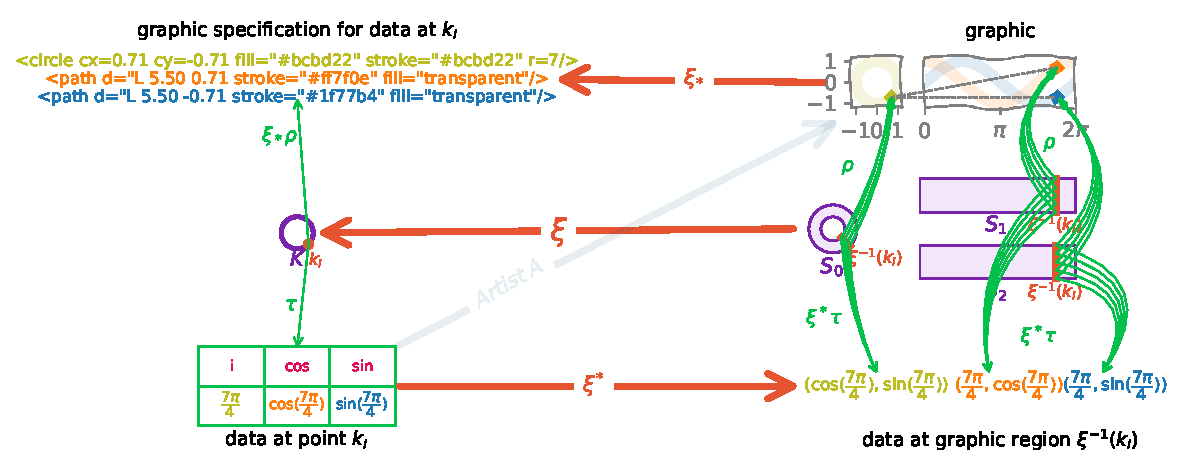
\includegraphics[width=1\textwidth]{xi_diagram.pdf}
  \caption{The data  \dsectionc\ consists of the $sin$ and $cos$ functions over a unit circle base space, which here are circle and two line plots generated from the graphic specification \gsectionc\. The index map \vindexc\ keeps track of which part of the circle, sin, and cosine plots correspond to which point on the unit circle. For example the orange bands on $\gbase_0, \gbase_1, \gbase_2$ map to the orange point $\dbasepoint_i$. The pushforward $\vindexpushc$ matches each point in the data space to the specification of the graphic at that point, here illustrated as an svg-like specification. The pullback $\vindexpull$ matches each point in the graphic space to the data over that point, and as shown often the same data point maps to multiple graphic spaces (and their corresponding pixels). The artist \vartistc\ is the function
  that transforms data into a graphic and is introduced in \autoref{sec:artist}.
  \label{fig:atct:morphisms:sheaf}}
\end{figure*}

As illustrated in \autoref{fig:atct:morphisms:sheaf}, modeling the data and graphic containers as sheaves and constructing structure preserving maps between the indices provides a method of precisely describing the which data values belong with which graphical representations. The $(\dbasepoint_i, \gbase_i)$ pairing expressed in \autoref{eq:atct:xi} establishes that there is a correspondence between data at an index $\dbasepoint_i$ and graphics generated at $\gbase_i$. In \autoref{fig:atct:morphisms:sheaf}, one example of this correspondence is the the orange bands on $\gbase_0, \gbase_1, \gbase_2$ that correspond to the orange point $\dbasepoint_i$. Because of this correspondence and the properties of sheaves, we can construct a graphic specifications for each data index $\vindexpush\gsection$; in \autoref{fig:atct:morphisms:sheaf}  $\vindexpush\gsection(\dbase_i)$ a svg-like spec describing the piece of the circle, sin, and cosine curves generated for the data at the point \dbasepointc\. We can also retrieve the data $\vindexpull\dsection_{\vindexpre(\dbasepoint)}$ that is being visualized by each specific part of the graphic, which in \autoref{fig:atct:morphisms:sheaf} is the section $\dsection(\dbasepoint_i)$.

\section{Codifying Structure Preservation}
\label{sec:artist}
%%Representing data and graphics as fiber bundles means that the fields and topology of the dataset and graphic can be described in a uniform way. Implementing data containers as sheaves means that visualization components can be designed under the assumption that subsets of the data have the same properties as the whole sets. Maintaining an index between graphic space and data space facilitates transporting graphic and data access functions (\gsection, \dsection) to data and graphic space (\vindexpush\gsection, \vindexpull\dsection) respectively. -> not sure if
Data visualization components are implementing a structure preserving mapping from a dataset to a graphic, which in the framework presented in this paper is a function from data to graphic sheaf. We call these structure preserving functions \textcolor{artist}{Artists}\footnote{Artists are named for the Artist class in Matplotlib. Artist is the parent class of all the objects that assemble and manage visual elements such as points, lines, and shapes.}:


\begin{equation*}
  \begin{tikzcd}
    & {} \arrow[dd, "\texttt{artist}" description, Rightarrow, shift left=3.65, shorten <= .7em, shorten >= .7em, color=artist, font=\Huge]
    & \\ {\scriptstyle\textcolor{base}{\texttt{topology}}}
      \arrow[rr, "\texttt{graphic}"', bend right, color=sheaf, font=\huge] \arrow[rr, "\texttt{data}", bend left, color=sheaf, font=\huge] &
    & {\scriptstyle\textcolor{base}{\texttt{topology}}\textcolor{section}{\rightarrow} \textcolor{fiber}{\texttt{fields}}} \\
    & {}                                              &
\end{tikzcd}
\end{equation*}

%move this down to what is math section
\begin{align}
  \label{eq:artist:hom_transport}
  \vartistc:& \cgamma{\dbasec}{\dtotalc}\textcolor{artist}{\rightarrow} \imartist{\gbasec}{\gtotalc}, \imartist{\gbasec}{\gtotalc} \subset \cgamma{\gbasec}{\gtotalc}
\end{align}


The output of an artist \vartist\ is a restricted subset of graphic sections $\imartist{\gbasec}{\gtotalc}$ that are, by definition, only reachable through a structure preserving artist:
\begin{equation}
  \label{eq:artist:output}
  \imartist{\gbasec}{\gtotalc} \coloneqq\\
  \{\gsectionc \mid\;\exists\;\dsectionc \in \cgamma{\dbasec}{\dtotalc}\;s.t.\;
  \vartistc(\dsectionc) = \gsectionc,\; \vindexc(\gbasec) = \dbasec \}
\end{equation}
We define this subset because the space of all sections $\cgamma{\opensetg}{\gtotal\restriction_{\openset}}$ is every possible way of setting pixels on an H base space, including non structure preserving settings such as setting all the pixels the same color.

While Artists are defined as maps going from data over \dbase\ to graphic over \gbase\, they are compatible with maps defined solely over \dbase\ or \gbase. This is because when a sheaf is equipped with transport functors (\vindexpush, \vindexpull), maps between sheaves over one space $Hom _{\sheaf_{\dbase}}$ are isomorphic to maps between sheaves over the other space $Hom _{\sheaf_{\gbase}}$\cite{harder2008lectures}:

\begin{equation}
  \label{eq:artist:homset}
  \begin{tikzcd}[column sep=50]
 \cgamma{\opensetc}{\vindexpushc\gtotalc\restriction_{\opensetc}}
& \cgamma{\opensetgc}{\gtotalc\restriction_{\opensetgc}}
\arrow[l, "\vindexpushc"', color=functor]                                          \\
\cgamma{\opensetc}{\dtotalc\restriction_{\opensetc}}
\arrow[r, "\vindexpullc", color=functor]
\arrow[u, "\textcolor{set}{Hom}_{\sheafc_{\dbasec}}", color=homset]
\arrow[ru, "{\textcolor{set}{Hom}_{\sheafc_{\dbasec},\sheafc_{\gbasec}}}", color=homset]
&
\cgamma{\opensetgc}{\vindexpullc\dtotalc\restriction_{\opensetgc}}
\arrow[u, "\textcolor{set}{Hom}_{\sheafc_{\gbasec}}"', color=homset]
\end{tikzcd}
\end{equation}
Both $Hom _{\sheaf_{\dbase}}$ and $Hom _{\sheaf_{\gbase}}$ are compatible, via composition with \vindex, with a mapping from data sheaf in data space to graphic sheaf in graphic space $Hom _{\sheaf_{\dbase}, \sheaf_{\gbase}}$. Artists are a subset of structure preserving functions in $Hom _{\sheaf_{\dbase}, \sheaf_{\gbase}}$ \textcolor{artist}{Artists}. For example, the artist in \autoref{fig:atct:morphisms:sheaf} is the blue arrow that converts $(i, \sin(i), cos(i))$ into the corresponding sections of the circle and lines.

The commutativity of \autoref{eq:artist:homset} means that an artist over data space $\vartist_{\dbase}: \dsection \mapsto \vindexpush \gsection$, an artist over graphic space $\vartist_{\gbase}: \vindexpull \dsection \mapsto \gsection$, and an artist $\vartist: \dsection \mapsto \gsection$ are equivalent. Specifically, given \autoref{eq:atct:sheaf:pullback_hover} (\vindexpull) and \autoref{eq:atct:sheaf:pushforward_select} (\vindexpush), $\vartist_{\dbase}(\dsection(\dbasepoint)) = \vartist_{\gbase}(\vindexpull\dsection(\gbasepoint)) = \vartist(\dsection(\dbasepoint)$ when $\vindex(\gbasepoint) = \dbasepoint$. The ability to shift base spaces using adaptors (\vindexpush, \vindexpull) allows a developer to specify structure preserving visualization components in data space, graphic space, or a mix of both depending on what is optimal for the specific use case. For example, mapping a line to a color in data space, but drawing the line in graphic space so that it can be dynamically resampled based on panning and zooming.

Because Artists can be constructed as morphisms of sheaves over either \dbase\ or \gbase\ through the application of pushforward and pullback functors (\vindexpush, \vindexpull), they are natural transformations \cite{bradleyWhatNaturalTransformation}.
\begin{definition}\label{def:natural-transform}
  Given two functors $F, G: \mathcal{C}\rightarrow \mathcal{D}$, a \textbf{natural transformation} $\alpha: F \rightarrow G$ is a function which assigns to each object $c$ of $\mathcal{C}$ a morphism $\alpha_c:F(input) \rightarrow G(c), G(c) \in \mathcal{D}$, in such a way that for every morphism $f:c \rightarrow c^\prime, c^\prime \in \mathcal{C}$, the morphisms in $\mathcal{D}$ commute such that $\alpha_c^{\prime}(F(f)(F(c))) = G(f)(\alpha_c(F(c))$. When this holds, $\alpha_{c}$ is \textit{natural} in $c$.\cite{maclaneCategoriesWorkingMathematician2013}.
\end{definition}.

This means that the structure on $\mathcal{C}$, as defined by its input objects $c \in \mathcal{C}$ and morphisms $f: c \rightarrow c^\prime$ are preserved in the output of the functors $F, G$ and by maps between functors $\alpha$. The artist \vartist\ is the natural transform mapping the sheaf functors $\sheaf_{data} \rightarrow \sheaf_{graphic}$, which both have the signature $\dbase^{op} (\gbase^{op})\rightarrow \texttt{set}$ \autoref{def:atct:presheaf}. This preservation of the structure of the input in the output encapsulates the structure preservation discussed in \autoref{sec:related-work:equivariance} and serves as the basis for describing structure preservation in \autoref{sec:artist:equiv}. Because the Artist is a natural transform and natural transforms are maps of functors that take the same input object and return objects in the same category\cite{milewskiCategoryTheoryProgrammers}, the artist signature can be formulated as:
 \begin{align*}
  \textcolor{artist}{\texttt{Artist}}:&(\textcolor{section}{\texttt{dataset}}: \textcolor{base}{\texttt{topology}}\textcolor{section}{\rightarrow} \textcolor{fiber}{\texttt{fields}}) \\
  \textcolor{artist}{\rightarrow} & (\textcolor{section}{\texttt{graphic}}: \textcolor{base}{\texttt{topology}}\textcolor{section}{\rightarrow} \textcolor{fiber}{\texttt{fields}})
 \end{align*}
where \texttt{topology} and \texttt{field} are meta classes of compatible types.

\subsection{Homeomorphism}

As introduced in \autoref{sec:related-work:continuity}, the topology of a dataset is preserved in the visualization if there is a homeomorphic map between the graphic and data indexing space. Because multiple graphics can correspond to one data record and every graphic must have a corresponding record \cite{tufteVisualDisplayQuantitative2001,ziemkiewiczEmbeddingInformationVisualization2009}, we define \textcolor{functor}{indexing look up functor} \vindexc\ as a deformation retraction\cite{hatcherAlgebraicTopology2002} of the graphic indexing space \gbase\ into the data indexing space \dbase. This means that every point in \gbase\ can be mapped, non-uniquely, to a point in \dbase\:

\begin{equation}
  \vindexc: \dbasec \times I \rightarrow \dbasec\;s.t\;\vindexc(\gbasepointc) = \dbasepointc\;\forall \dbasepointc \in \gbasec
\end{equation}
The graphic indexing space is defined as the data space multiplied by an identity $\gbase = \dbase\times I$ because it allows us to encode the data index into the graphic index. For example, for a 2D space the graphic basepoint is defined as $\gbasepoint=(\alpha,\beta) \in \dbasepoint_i\times I$ . This means that the first coordinate $\alpha=\dbasepoint_i$ provides a lookup into the data space and the second coordinate is a point on the interval $\beta \in I$ and together they are input into the graphic function $\gsection(\gbasepoint)$ which returns how the pixel at $\gbasepoint$ is set.

\begin{figure}[H]
  \includegraphics[width=1\columnwidth]{xi_zoom.pdf}
  \caption{The function $\xi$ maps each point in each orange band on each graphic indexing space $\gbase_0, \gbase_1, \gbase_2$ to the same point $\dbasepoint_i$ in the circle $\dbase$. As shown in \autoref{fig:atct:morphisms:sheaf}, the parts of the graphic indexed by the orange bands are visualizing parts of the record at $\dbasepoint_i$ \label{fig:artist:xi}}
\end{figure}

In \autoref{fig:artist:xi} each orange band is defined as $\frac{7\pi}{4}\times [0,1]$ such that each point on each band maps to the same point $\vindex|_{\frac{7\pi}{4}\times [0,1]} = \frac{7\pi}{2}$. As illustrated in \autoref{fig:atct:morphisms:sheaf}, each band acts as an indexer into its corresponding image because the section \gsection\ takes as input coordinates $(\frac{7\pi}{4}, \beta), \beta \in [0,1]$ in each orange band and returns the settings for the pixel it maps into. As illustrated in \autoref{fig:artist:xi}, the definition of $\vindex$ allows for some flexibility in the shape of $\gbase$. An annulus $\gbase_0$ is used for the green circle in \autoref{fig:atct:morphisms:sheaf} because that cyclical structure is in the graphic and in \dbase\, but rectangles $\gbase_1, \gbase_2$ are used for the $\sin$ and $\cos$ curves because they are linear. Despite discarding the cyclical information embedded in \dbase\, the spaces $\gbase_1$ and $\gbase_2$ are structure preserving because they satisfy the constraint on \vindex\ that every graphic element maps back into a data element \cite{ziemkiewiczEmbeddingInformationVisualization2009}.

Because the artist is specified as a natural transform (\autoref{def:natural-transform}) on sheaves, the artist expects that subsets of the dataset have the same properties as the whole dataset when the artist preserves the presheaf and sheaf constraints (\autoref{def:atct:presheaf}, \autoref{def:atct:sheaf}) when mapping data into graphics. Preserving the presheaf constraints means that the set of possible visualizations for a larger set of values must include all visualizations for a subset of those values  $\vartist(\Gamma(\dbase_1, \dtotal)) \xrightarrow{i^*} \vartist(\Gamma(\dbase_2, \dtotal))$ when more values may exist on the subset of the index $\dbase_2 \xhookrightarrow{i} \dbase_1$. While the curves in \autoref{fig:atct:presheaf} are meant as stand-ins for the data, they also serve to illustrate that the relationship is identical in the graphic space. The artist preserves the \textit{locality} axiom in that identical datasets $\dsection^{a} = \dsection^{b}$ generate identical specifications $\vartist(\dsection^a) = \vartist(\dsection^b)$. The artist respects \textit{gluing} in that graphics are composable, as described in \autoref{sec:artist:operators}, such that a set of artists that generate graphics for parts of a dataset are equivalent to an artist that generates a graphic for the whole dataset. Managing subsets of data and on demand data in a structure preserving way is necessary to support visualizing streaming data \cite{krstajicVisualizationStreamingData2013} and techniques that rely on shifting or resampling the indexing space, such as  panning and zooming \cite{NekrasovskiEvaluationPanZoom2006}.

\subsection{Equivariance}
\label{sec:artist:equiv}
As introduced in \autoref{sec:related-work:equivariance}, data and the corresponding visual encoding are expected to have compatible structure such that actions (\autoref{def:related-work:action}) on data and graphic are symmetric. We generalize from binary operations to a family of actions $\dfunc \in \dfuncset$ on the sheaf $\sheaf_{\dbase, \dtotal}$ because that allows for expanding the set of allowable transformations on the data beyond a single operator. We describe the changes on the graphic side as changes in \textcolor{monoid}{measurements} \measurec\ of visual components. A superset of the Bertin visual variables \cite{bertinIIPropertiesGraphic2011}, measurable components are scaler or vector components of the rendered graphic that can be quantified, such as the color, position, shape, texture, or rotation angle of the graphic. For example, a measurement of a scatter marker could be its color (e.g. red) or its x position (e.g. 5).


\subsubsection{Mathematical Structure of Data}
\label{sec:artist:equivariant:data}
\note{something something rotation etc}
We separate data transformations into two components, transformations on the base space $(\dfunchc, \dfuncpullc)$ and transformations on the fiber space $\dfunctc$.

\begin{equation}
  \label{eq:artist:sheaves:monoid_morphism}
  \begin{tikzcd}
    \cgamma{\opensetc}{\dtotalc\restriction_{\opensetc}}
    \arrow[rr, "\dfuncpullc", color=action, maps to] &  &
    \cgamma{\opensetc^{\prime}}{\dfuncpullc\dtotalc\restriction_{\opensetc^{\prime}}} &
    \cgamma{\opensetc^{\prime}}{\dfuncpullc\dtotalc\restriction_{\opensetc^{\prime}}}
    \arrow[dd, "\dfunctc", color=action] \\
     &  & &       \\
    \opensetc
    \arrow[uu, maps to,color=sheaf]  &  & \opensetc^{\prime}
    \arrow[ll, "\dfunchc"', color=action, maps to]
    \arrow[uu, maps to, color=sheaf] & \cgamma{\opensetc^{\prime}}{\dfuncpullc\dtotalc\restriction_{\opensetc^{\prime}}}
    \end{tikzcd}
\end{equation}
The base space transformation transforms one openset object $\openset^{\prime}$ to another object $\openset$, and the pullback functor transports the entire set of sections $\Gamma(\openset, \dtotal\restriction_{\openset})$ over the new base space $\Gamma(\openset^{\prime}, \dfuncpull\dtotal\restriction_{\openset^{\prime}})$. The fiber transformation transforms a single section $\dfuncpull\dsection$ to a different section $\dfuncpull\dsection$.

\paragraph{\textbf{Topological structure}}
\noindent
The base space transformation is a point wise continuous map from one open set to another open set in the same base space
\begin{equation}
  \label{eq:atct:morphism:base}
 \dfunchc: \dbasepointc^{\prime}\mapsto \dbasepointc
 \end{equation}
such that $\openset, \openset^{\prime} \subseteq \dbase$. This means $\openset$ and $\openset^{\prime}$ are of the same topology type. To correctly align the sections with the remapped base space, there is a a corresponding section pullback function
\begin{equation}
  \label{eq:atct:morphism:basepull}
  \dfuncpullc \dsectionc \restriction_{\opensetc^{\prime}}: \dsectionc\restriction_{\opensetc^{\prime}} \mapsto \dsectionc \restriction_{\opensetc^{\prime} \circ \dfunchc}
\end{equation}
such that $\dsection|_{\openset} = \dfuncpull\dsection|_{\opensetc^{\prime}}$ because $\dsection|_{\openset} = \dsection|_{\dfunch(\opensetc^{\prime})}$. This means that the base space transformation  $\dfunch(\dbasepoint^{\prime}) = \dfunch(\dbasepoint)$ such that
\begin{equation}
  \label{eq:atct:morphism:verify_base}
  \dsectionc(\dbasec) = \dfuncpullc\dsectionc(\dbasepointc^{\prime}) = \dsectionc(\dfunchc(\dbasepointc^{\prime}))
\end{equation}
which means that the index of the record changes from $\dbasepoint$ to $\dbasepoint^{\prime}$ but the values in the record are unmodified.

\paragraph{\textbf{Records}}
As introduced in \autoref{eq:artist:sheaves:monoid_morphism}, the fiber transformation $\dfunctc$ is a change in section
\begin{equation}
  \label{eq:atct:morphism:fiber}
  \dfunctc: \dfuncpullc \dsectionc \restriction_{\opensetc^{\prime}} \mapsto \dfuncpullc \dsectionc^{\prime} \restriction_{\opensetc}
\end{equation}
where $\dsection, \dsection^{\prime} \in \Gamma(\openset^{\prime}, \dfuncpull\dtotal\restriction_{\openset^{\prime}})$. Since $\dfunct$ maps from one continuous function to another, it must itself be continuous such that
\begin{equation}
  \label{eq:atct:morphism:fiber:continuity}
   \lim\limits_{x \rightarrow \dbasepointc^{\prime}}\dfunctc(\dfuncpullc\dsectionc(x)) =  \dfunctc(\dfuncpullc\dsectionc(\dbasepointc^{\prime}))
\end{equation}
As mentioned in \autoref{sec:atct:fb:fiber}, $\dfunct$ is also
a morphism on the fiber category $\dfunct \in Hom(\dfuncpull\dfiber\restriction_{\dbasepoint^{\prime}},\dfuncpull\dfiber\restriction_{\dbasepoint^{\prime}})$ restricted to a point $\dbasepoint^{\prime} \in \openset^{\prime}$. This means $\dfunct$ has to satisfy the properties of a morphism (\autoref{def:atct:category})
\begin{itemize}
  \item \textit{closed}: $\dfunctc(\dfuncpullc\dsectionc(\dbasepointc^{\prime})) \in \dfiberc$
  \item \textit{unitality}: $\dfunctc(id_{\dfiberc}(\dfuncpullc\dsectionc(\dbasepointc^{\prime}))) = id_{\dfiberc}(\dfunctc(\dfuncpullc\dsectionc(\dbasepointc^{\prime})))$
  \item \textit{composition and associativity}: \\
  $\dfunctc(\dfunctc(\dfuncpullc\dsectionc(\dbasepointc^{\prime}))) = (\dfunctc\circ\dfunctc)(\dfuncpullc\dsectionc(\dbasepointc^{\prime}))$
\end{itemize}

Additionally, $\dfunctc$ must preserve any features of $\dfiber$, such as operators that are defined as part of the structure of $\dfiber$. Examples of testing that $\dfunctc$ preserves the operations, and therefore structure, of the Steven's measurement scales are shown in \autoref{tab:appendix:summary:stevens}. We do not provide a general rule here because these constraints are defined with respect to how specific properties of the mathematical structure of individual fields $\dfiber$ are expected to be preserved rather than as a general consequence of $\dfunctc$ being a section map and morphism of the category.

\paragraph{\textbf{Topological structure and records}}
\noindent We define a full data transformation as one that induces both a remapping of the index space and a change in the data values
\begin{equation}
  \label{eq:atct:morphism:all}
  \dfuncc: \dsectionc\restriction_{\opensetc} \mapsto \dsectionc^{\prime}\restriction_{\opensetc} \circ \dfunchc
\end{equation}
which gives us an equation that can express transformations that have both a base space change and a fiber change.

The data transform \dfunc\ is composable
\begin{equation}
  \dfuncc = (\dfunchc, \prod\limits_{i=0}^{n}\dfunctc_i)
\end{equation}
if each (identical) component base space is transformed in the same way $\dfunch$ and there exists functions $\dfunc_{a,b}: \dtotal_a \times \dtotal_b \rightarrow \dtotal_a \times \dtotal_b$, $\dfunc_{a}: \dtotal_a \rightarrow \dtotal_a$ and $\dfunc_{b}: \dtotal_b \rightarrow \dtotal_b$ such that $\pi_a \circ \dfunc_a = \dfunc_{a,b} \circ \pi_a$ and $\pi_b \circ \dfunc_b = \dfunc_{a,b} \circ \pi_b$ then $\dfunc_{a,b} = (\dfunc_a, \dfunc_b)$. This allows us to define a data transform where each fiber transform $\dfunct_{i}$ can be applied to a different fiber field $\dfiber_i$.

\begin{figure}[H]
  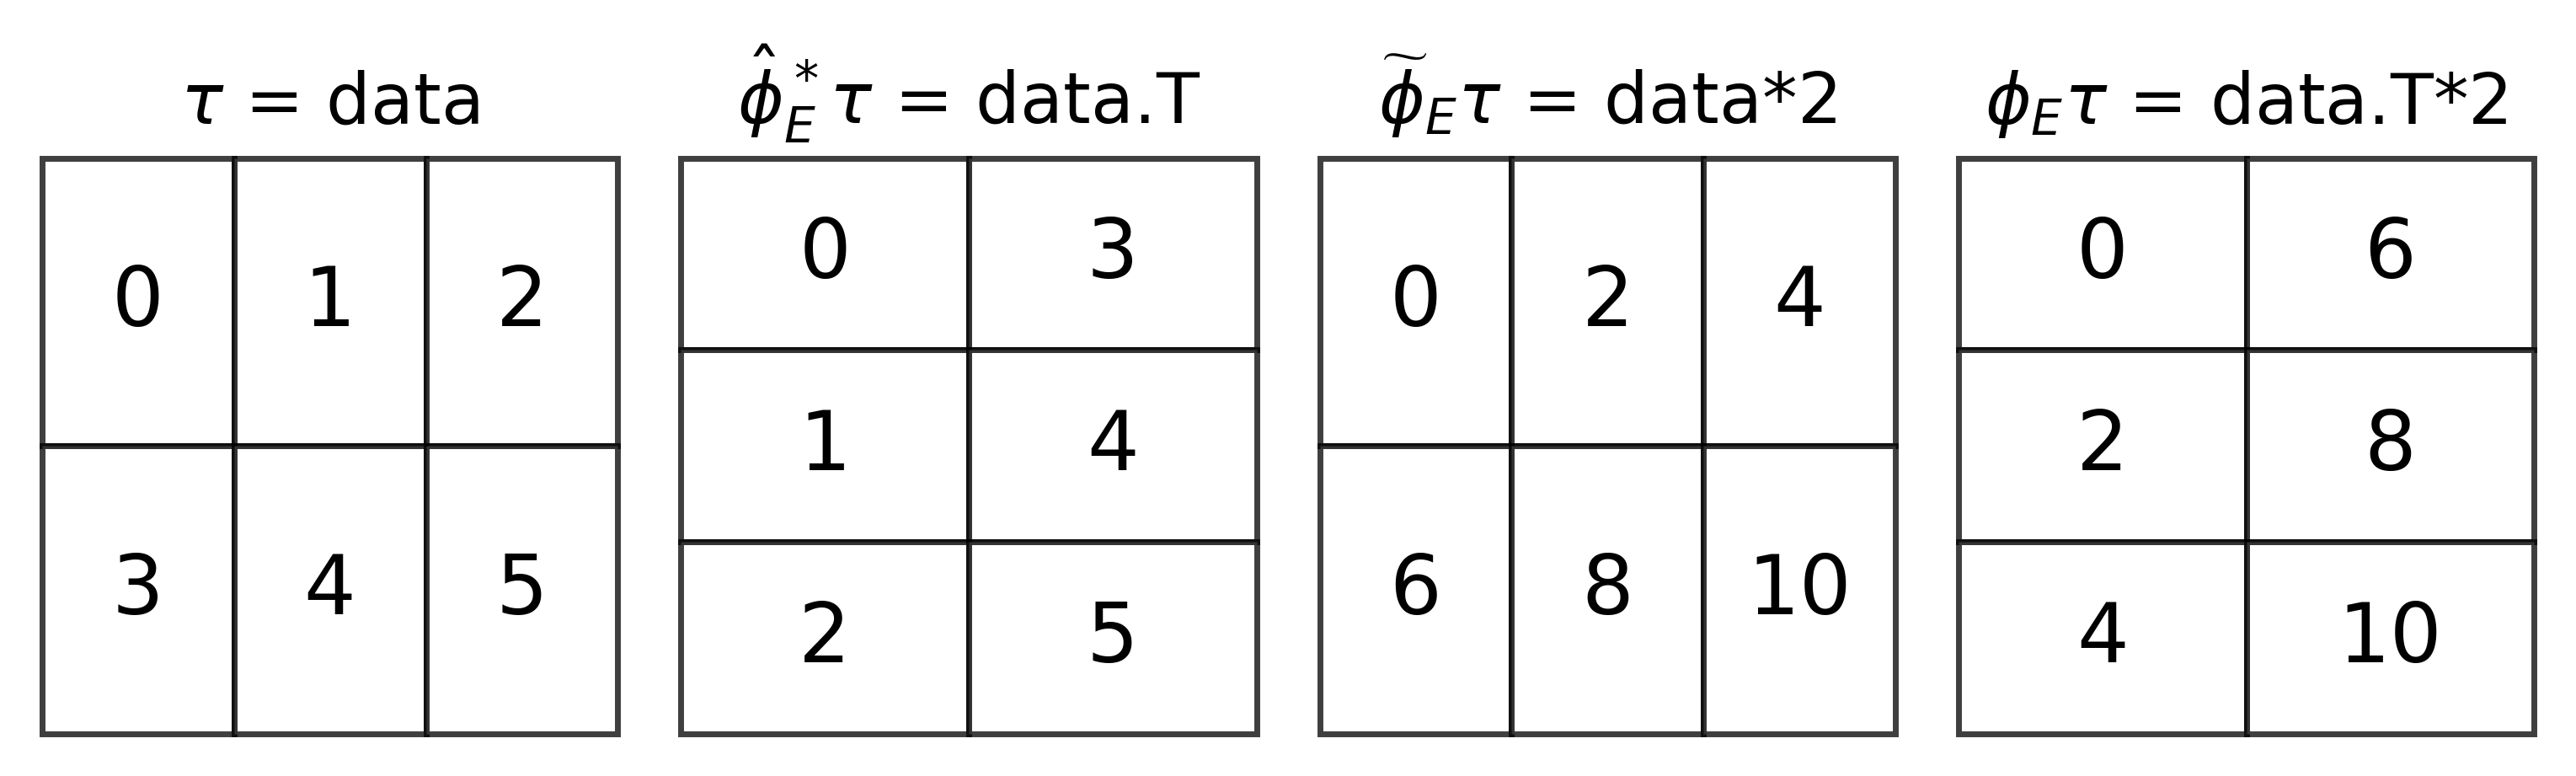
\includegraphics[width=\columnwidth]{phi.png}
  \caption{Values in a data set can be transformed in three ways: $\dfunch$-values can change position, .e.g transposed;  $\dfunct$-values can change, e.g. doubled; $\dfunc$ - values can change position and value  \label{fig:atct:phi}}
\end{figure}
\autoref{fig:atct:phi} provides an example of a transposition base space change \dfunch, a scaling fiber space change \dfunct, and a composition of the two \dfunc\ applied to each data point $x_{\dbasepoint} \in \texttt{data}$. In the transposition only case, the values in $\dfuncpull\dsection$ retain their neighbors from $\dsection$ because \dfunc\ does not change the continuity. Each value in $\dfuncpull\dsection$ is also the same as in $\dsection$, just moved to the new position. In $\dfunct\dsection$, each value is scaled by two but remains in the same location as in $\dsection$. And in $\dfunc\dsection$ each function is transposed such that it retains its neighbors and all values are scaled consistently.


\subsubsection{Equivariant Artist}
\label{sec:artist:equivariant:artist}
We formalize this structure preservation as equivariance, which is that for every morphism on the data $(\dfunch_{\dtotal}, \dfunct_{\dtotal})$ there is an equivalent morphism on the graphic  $(\dfunch_{\gtotal}, \dfunct_{\gtotal})$ The artist is an equivariant map if the diagram commutes for all points $\gbasepointc^{\prime}\in \gbasec^{\prime}$

\begin{equation}
  \label{eq:artist:equivariance}
  \begin{tikzcd}[ampersand replacement=\&, column sep=small]
  \cgamma{\dbasec}{\dtotalc}
  \arrow[rrr, "\vartistc", color=artist]
  \arrow[d, "\dfuncpullc_{\dtotalc}"', color=action]
  \& \& \&
  \imartist{\gbasec}{\gtotalc}
  \arrow[d, "\dfuncpullc_{\gtotalc}", dotted] \\
  \cgamma{\dbasec^{\prime}}{\dfuncpullc_{\dtotalc}\dtotalc}
  \arrow[dd, "\dfunctc_{\dtotalc}"', color=action] \&
  \dbasec
   \&
  \gbasec
  \arrow[l, "\vindexc"', color=functor]
  \&
  \imartist{\gbase^{\prime}}{\dfuncpullc_{\gtotalc}\gtotalc}
  \arrow[dd, "\dfunctc_{\gtotalc}", dotted, color=action] \\
  \&
  \dbasec^{\prime}
  \arrow[u, "\dfunchc_{\dtotalc}", color=action]
  \&
  \gbasec^{\prime}
  \arrow[l, "\vindexc"', color=functor]
  \arrow[u, "\dfunchc_{\gtotalc}"', dotted, color=action]
  \& \\
  \cgamma{\dbasec^{\prime}}{\dtotalc^{\prime}}
  \arrow[rrr, "\vartistc", color=artist]
  \& \& \&
  \imartist{\gbasec^{\prime}}{\gtotalc^{\prime}}
  \end{tikzcd}
\end{equation}
such that starting at an arbitrary data point $\dsectionc(\dbasepointc)$ and transforming it into a different data point and then into a graphic
\begin{equation*}
  \vartistc(\dfunctc_{\dtotalc}(\dsectionc(\dfunchc_{\dtotalc}(\vindexc(\gbasepointc^{\prime}))))) = \dfunctc_{\gtotalc}(\vartistc(\dsectionc(\vindexc(\dfunchc_{\gtotalc}(\gbasepointc^{\prime})))))
\end{equation*}
is equivalent to transforming the original data point into a graphic and then transforming the graphic into another graphic. The function $\dfunch_{\gtotal}$ induces a change in graphic generating function that matches the change in data. The graphic transformation $\dfunch_{\gtotal}$ is difficult to define because by definition it acts on a single record, for example a pixel in an idealized 2D screen.

Instead, we define an output \textcolor{action}{verification} function $\extractmc$ that takes as input the section evaluated on all the graphic space associated with a point $\gsection_{\vindexpre\restriction_{\dbasepoint}}$ and returns the corresponding \textcolor{action}{measurable visual components} $\measurec_{k}$. \note{formall define M as a space of measurements }
\begin{equation}
  \label{eq:artist:actual}
  \extractmc: (\gsectionc \circ \vindexpre) \mapsto (\dbasec \xrightarrow{\extractmc_{\gsectionc}} \measurec)
\end{equation}
The measurable elements can only be computed over the entire preimage because these aspects, such as thickness or marker shape, refer to the entire visual element.
\begin{equation}
  \label{eq:artist:inout:diagram}
  \begin{tikzcd}[row sep=huge]
    \cgamma{\dbasec}{\dtotalc}
    \arrow[rr, "\vartistc", color=artist]
    \arrow[d, "\equivc"', color=monoid] &  &
    \imartist{\gbasec}{\gtotalc}
    \arrow[d, "render"]
    \arrow[lld, "\extractmc"', color=monoid, dashed] \\
    {\textcolor{set}{Hom}(\dbasec, \measurec)}  &  & visualization
    \arrow[ll, "measure",]
    \end{tikzcd}
\end{equation}
The extraction function is equivalent to measuring components of the rendered image $\extractm = measure\circ render$, which means an alternative way of implementing the function when $\gbase$ is not accessible is by decomposing the output into its measurable components.

We also introduce a function \equivc\ that maps data to the measurement space directly
\begin{equation}
\equivc: \dsectionc \mapsto (\dbase \xrightarrow{\equivc_{\dsectionc}} \measurec)
\end{equation}
such that $\equivc_{\dsection}(\dbasepointc)$ is the expected set of measurements $\measure_{\dbasepoint}$. The pair of \textcolor{monoid}{verification functions} (\equivc, \extractmc) can be used to test that the expected encoding $\equivb_{\dsection}$ of the data matches the actual encoding $\extractm_{\gsection}$
\begin{equation}
  \label{eq:artist:verification}
    \equivc(\dsectionc)(\dbasepointc) = \extractmc(\vartistc(\dsectionc))(\dbasepointc) = \extractmc(\gsectionc\circ\vindexprec)(\dbasepointc)=\measurec_{\dbasepointc}
\end{equation}

An artist is equivariant when changes to the input and output are equivariant. As introduced in \autoref{eq:atct:morphism:base}, the base space transformation \dfunch\ is invariant because $\dsection\restriction_{\openset} = \dsection\restriction_{\dfunch(\openset^{\prime})}$. This means that, for all points in the data $\dbasepoint \in \dbase$, the measurement should not change if only the base space is transformed
\begin{equation}
  \label{eq:atct:equivarance:verify:base}
  \equivc(\dsectionc)(\dfunchc(\dbasepointc^{\prime})) = \extractmc(\vartistc(\dsectionc))(\dbasepointc)
\end{equation}
On the other hand, a change in sections \autoref{eq:atct:morphism:fiber} induces an equivalent change in measurements
\begin{equation}
  \label{eq:atct:equivarance:verify:fiber}
  \equivc(\dfunctc(\dsectionc))(\dbasepointc) = \dfunctc_{\measure}(\extractmc(\vartistc(\dsectionc))(\dbasepoint))
\end{equation}
The change in measurements $\dfunctc_{\measure}$ is defined by the developer as the symmetry between data and graphic that the artist is expected to preserve.

\begin{figure}[H]
  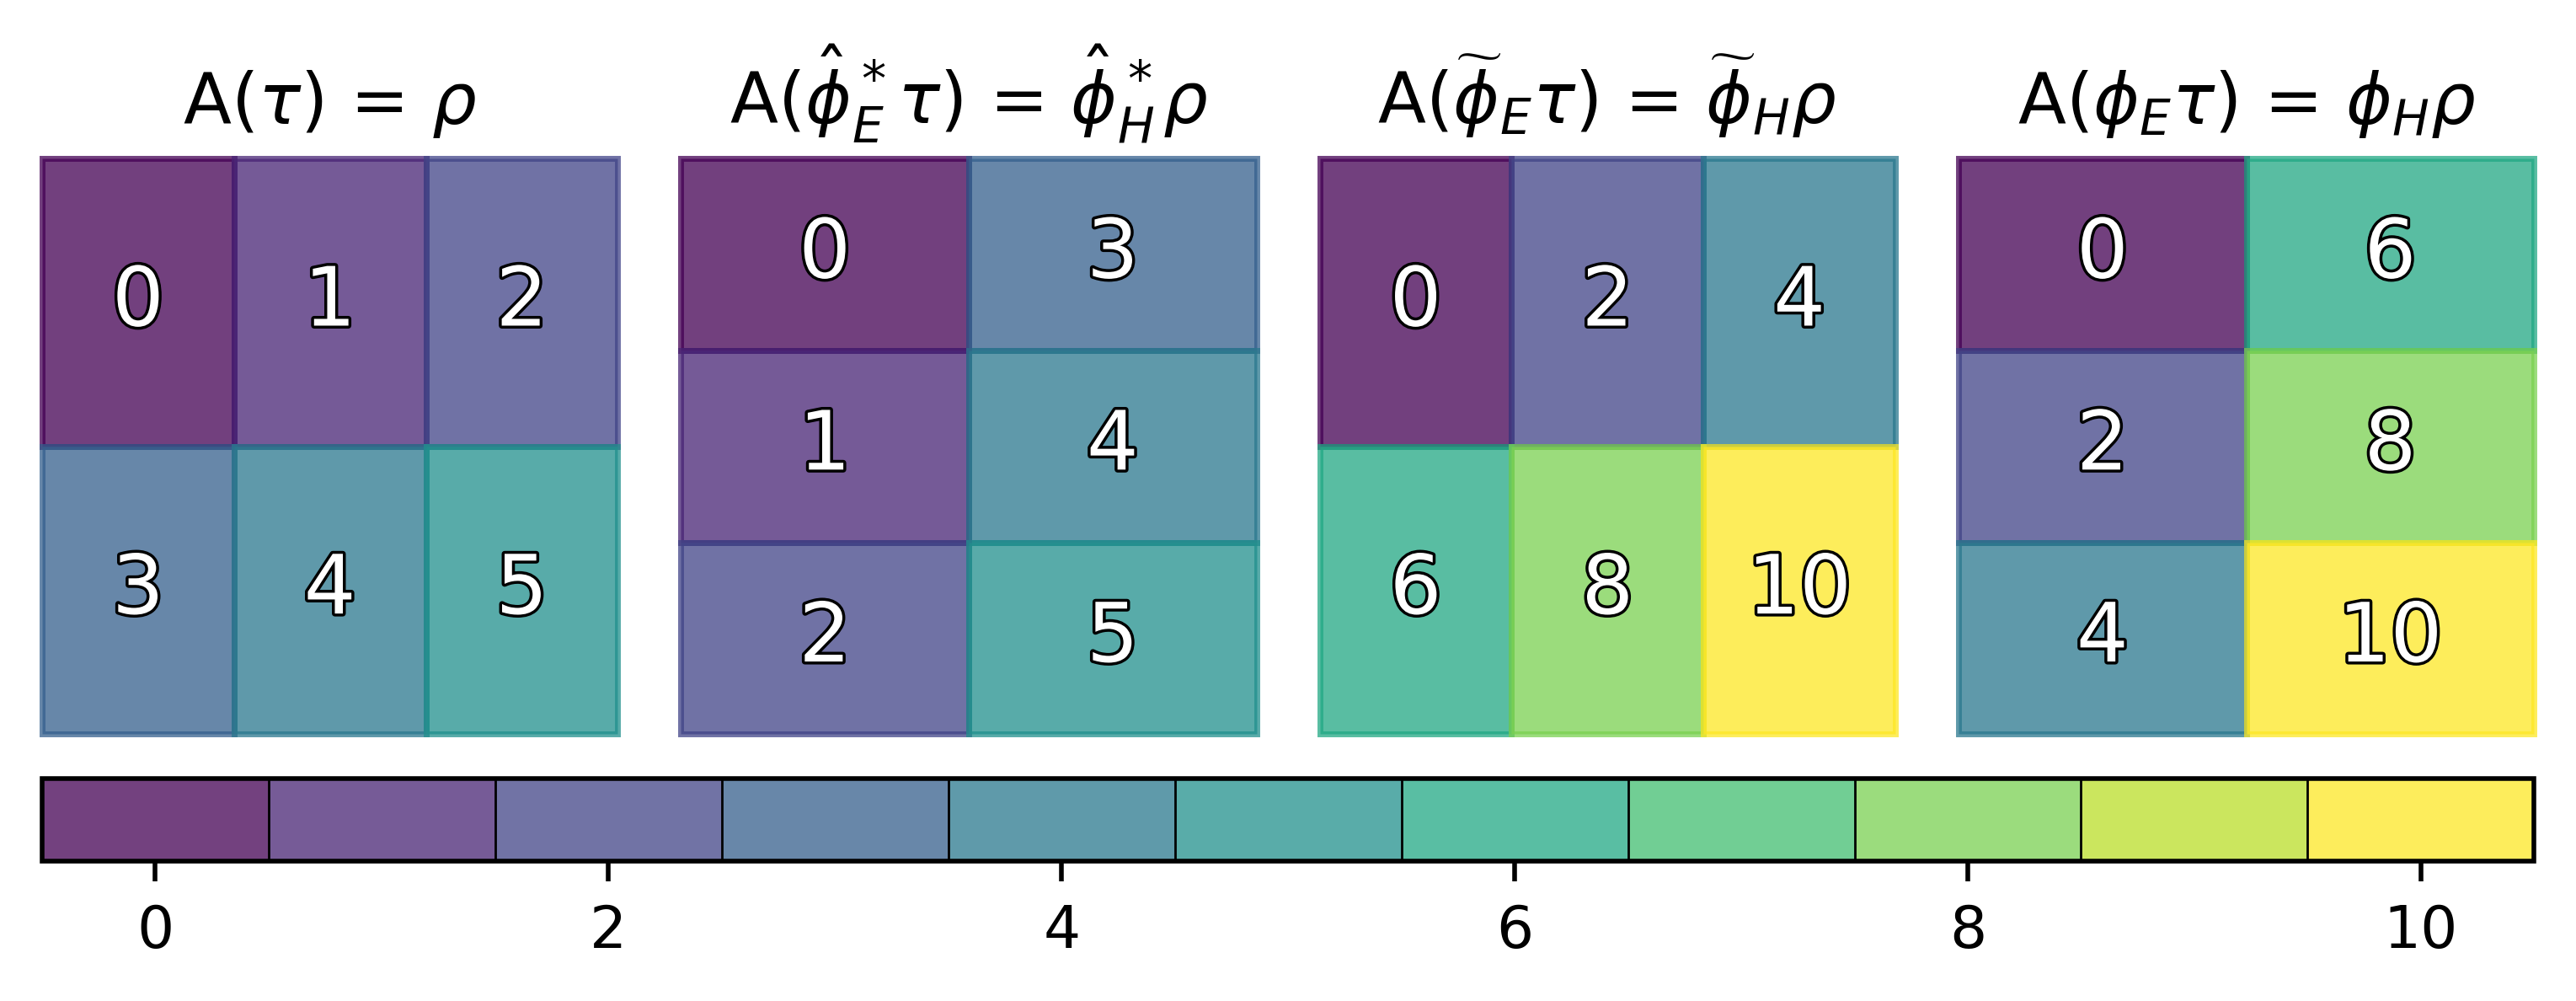
\includegraphics[width=1\columnwidth]{equivariance.png}
  \caption{This artist is equivariant because when the input data $\dsection$ is transposed, $\dfunch$, scaled $\dfunct$, and transposed and scaled $\dfunc$, the corresponding colored cells are transposed, scaled such that the color is moved two steps, and both transposed and scaled.
  \label{fig:artist:equivariance}}
\end{figure}

For example, in \autoref{fig:artist:equivariance}, the measurable variable is color. This is a visual representation of the data shown in \autoref{fig:atct:phi}, and as such the equivariant transformations are an equivalent transposition and scaling of the colors. This visualization is equivariant with respect to base space transformations, as defined in \autoref{eq:atct:equivarance:verify:base}, because the color values at the new position at the old position $measure_\dbasepoint^{\prime} = \measure_{\dbasepoint}$. This visualization is also equivariant with respect to fiber wise transformations, as defined in \autoref{eq:atct:equivarance:verify:fiber}, because the colors are consistently scaled in the same was the data. For example, the values that have become 2 and 4 in the $\dfunctc$ and $\dfunc$ panels are colored the same as the original 2 and 4 values in the first panel. The equivariance in this visualization is composable, as shown in the colors being both transposed and scaled correctly in the $\dfunc$ panel.

\subsection{Composing Artists}\label{sec:artist:operators}
\note{addition: intersections mapped same, multiplication: fibers mapped same}
\note{large big data glued together correctly}
A common use of category theory in software engineering is the specification of modular components \cite{wielsManagementEvolvingSpecifications1998} such that we can build systems where the structure preserved by components is preserved in the composition of the components. This allows us to express that an artist that works on a dataset can be composed of artists that work on sub parts of that dataset.


\subsubsection{Addition}
\label{sec:artist:addition}
We propose an addition operator that states that an artist that takes in a dataset can be constructed using artists that take as inputs subsets of the dataset
\note{adjoint equation is wrong, probably multiplication b/c using $k^a$ and $K^b$ to define the piecewise, disjoint union is coproduct}

\begin{equation*}
  \label{eq:artist:addition}
  \vartistc_{a+b}(\cgamma{\dbasec^{a} \sqcup_{\dbase^c} \dbasec^b}{\dtotalc}) \coloneqq \vartistc_{a}(\cgamma{\dbasec^{a}}{\dtotalc}) + \vartistc_{b}(\cgamma{\dbasec^{b}}{\dtotalc})
\end{equation*}
As introduce in $\autoref{eq:artist:hom_transport}$, the artist returns a function $\gsection$. We assume that the output space is a trivial bundle, which means that $\gsectionc \in Hom(\gbase, \gfiber)$ because the output specification is the same at each point $\gbase$. This allows us to make use of the hom set adjoint property\note{find citation}\
\begin{equation*}
  Hom(\gbase^{a} + \gbasec^b, \gfiber) = Hom(\gbase^{a}, \gfiber) + Hom(\gbase^b, \gfiber)
\end{equation*}
to define an artist constructed via addition as consisting of two distinct graphic sections
\begin{equation}
  \label{eq:artist:plus:output}
  \gsectionc(\gbasepointc) \coloneqq \begin{cases} \gsectionc^{a}(\gbasepointc) & \gbasepointc \in \vindexprec(\dbasec^{a}) \\
    \gsectionc^{b}(\gbasepointc) & \gbasepointc \in \vindexprec(\dbasec^{b})
  \end{cases}
\end{equation}
that are evaluated only if the input graphic point is an the graphic area that graphic section acts on.

One way to verify that these artists are composable is to check that the return the same graphic on points in the intersection $\dbase^{c}$.  Given $\dbasepointc_{a} \in \dbasec_{c} \subset \dbasec_{a}$ and $\dbasepointc_{b} \in \dbasec_{c} \subset \dbasec_{b}$, if $\dbasepointc_{a} = \dbasepointc_{b}$ then

\begin{equation}
  \label{eq:artist:plus:verify}
  \begin{split}
  &\vartistc_{a+b}(\dsectionc^{a+b}(\dbasepointc_{a})) \\
  & = \vartistc_{a}(\dsectionc^{a}(\dbasepointc_{a})) = \vartistc_{b}(\dsectionc^{b}(\dbasepointc_{b}))
  \end{split}
\end{equation}
 for all $\dbasepointc_{a}, \dbasepointc_{b} \in \dbasec_{a}\bigsqcup\limits_{\dbasec_{c}} \dbasec_{b}$

 \note{replace w/ a line plot w/markers}
 One example of an artist that is a sum of artists is a sphere drawer that draws different quadrants of a sphere $\vartist(\dsection) = \vartist_{1}(\dsection_{1}) + \vartist_{2}(\dsection_{2}) + \vartist_{3}(\dsection_{3}) \vartist_{4}(\dsection_{4})$. Given an input $\dbasepoint \in \dbase_4$ in the 4th quadrant, then the graphic section that would be executed is $\gsection_{4}$. If that point is also in the 3rd quadrant  $\dbasepoint \in \dbase_3$, then both artist outputs must return the same values $\gsection_{4}(\vindexprec(\dbasepoint)) = \gsection_{3}(\vindexprec(\dbasepoint))$.


\subsubsection{Multiplication}
\label{sec:artist:operator:multiplication}
\note{fiber product vs cartesian product}

In the trivial case where the base spaces are the same $\dbase^{a} = \dbase^{b} = \dbase$, this is equivalent to adding more fields to a dataset.

\begin{equation*}
  \label{eq:artist:multiplication}
  \vartistc_{a \times b}(\cgamma{\dbase}{\dtotalc^{a\times b}}) \coloneqq \vartistc_{a}(\cgamma{\dbasec}{\dtotalc^{a}}) \times \vartistc_{b}(\cgamma{\dbasec}{\dtotalc^{b}})
\end{equation*}

which following from an adjoint property of homsets \note{find citation and push this into a footnote or appendix maybe}
\begin{equation}
  Hom(\gbase, \gfiber) \times Hom(\gbase, \gfiber) = Hom(\gbase, \gfiber\times \gfiber)
\end{equation}

which means that the artists on the subsets of fibers can be defined
\begin{equation}
  \gsectionc^{a \times b} = \{\gsectionc^{a}(\gbasepointc), \gsectionc^{b}(\gbasepointc)\}, \gbasepointc \in \vindexprec(\dbasec)
\end{equation}
but that the signature of $\gsectionc^{a \times b}$ would be $\gbase \rightarrow \gfiber \times \gfiber$. Instead of having to special case the return type of artists that are compositions of multiple case, the hom adjoint \note{find cite} property
\begin{equation*}
  Hom(\gbase, \gfiber \times \gfiber) = Hom(\gbase+\gbase, \gfiber)
\end{equation*}
 means that multiplication can be considered as a special case of addition where $\dbase^{a} = \dbase^{b}$. While we discussed the trivial case in \autoref{sec:artist:addition}, there is no strict  requirement that $\dfiber^{a} = \dfiber^{b}$.

One way to verify that these artists are composable is to check that they encode any shared fiber $\dfiber^{c}$ in the same way.

\begin{equation}
  \begin{split}
    &\extractmc(\vartistc_{a\times b}(\dsectionc^{a\times b}(\dbasepointc)))\restriction_{\dfiberc^{c}}\\
    &=
    \extractmc(\vartistc_{a}(\dsectionc^{a}(\dbasepointc_{a})))\restriction_{\dfiberc^{c}} = \extractmc(\vartistc_{b}(\dsectionc^{b}(\dbasepointc_{b})))\restriction_{\dfiberc^{c}}
  \end{split}
\end{equation}

This expectation of using the same encoding for the same variable is a generalization of the concept of consistency checking of multiple view encodings discussed by Qu and Hullman \cite{hullmanKeeping2018}. This expectation can also be used to check that a multipart glyph is assembled correctly. For example, a box plot \cite{wickham40YearsBoxplots2011} typically consists of a rectangle, multiple lines, and scatter points; therefore a boxplot artist $\vartist_{boxplot} = \vartist_{rect} \times \vartist_{errors} \times \vartist_{line} \times \vartist_{points}$ must be constructed such that all the sub artists draw a graphic at or around the same x value.

\begin{figure}[H]
  \centering
  \includegraphics*[scale=.75]{qcom.png}
  \caption{The circle-line visual element can be constructed via $\gsection_{circle}$ + $\gsection_{line}$ functions that generate the circle and line elements respectively. This is equivalent to a $\gsection_{circle+line}$ function that takes as input the combined base space $\gbase_{circle} \sqcup \gbase_{line} = \gbase_{circle-line}$ and returns pixels in the circle-line element.  \label{fig:artist:operator}}
\end{figure}
There is no way to visually determine whether a visual element is the output of a single artist or a multiplied or added collection of artists. The circle-line visual element in \autoref{fig:artist:operator} can be a visual representation of a highlighted point intersecting with a line plot with the same fields. The same element can also be encoding some fields of a section in the circle and other fields of that section in the lines. \note{+*equive}
Although we have been discussing the trivial cases of adding observations or adding fields, this merging of artists in datasets can be generalized:
\begin{equation}
  \label{eq:artist:join_base_fiber}
  \vartistc(\cgamma{\mathop{\sqcup}_{i} \dbasec^{i}}{\mathop{\oplus}_{i}\dtotalc^{i}}) \coloneqq \sum_{i}
  \vartistc_{i}(\cgamma{\dbasec^{i}}{\dtotalc^{i}})
\end{equation}

As shown in \autoref{eq:artist:join_base_fiber}, bundles over a union of base spaces can be joined as a product of the fibers. This allows us to consider all the data inputs in a complex visualization as a combined input, where some sections evaluate to null in fields for which there are no values for that point in the combined base space $\dbasepoint \in \mathop{\sqcup}_{i} \dbase^{i}$ The combined construction of the data is a method for expressing what each data input has in common with another data input-for example the data for labeling tick marks or legends-
and therefore which commonalities need to be preserved in the artists that act on these inputs.

\note{explain why annotation is similar to brush/linking in operators section }

\subsection{Animation and Interactivity}


\begin{LaTeXdescription}
  \item[pan, zoom, scroll] sheaf: locality + gluing \autoref{def:atct:sheaf}
  \item[selection and hover] pushforward \autoref{eq:atct:sheaf:pushforward_select},  pullback \autoref{eq:atct:sheaf:pullback_hover}
  \item[brushing, linking, annotation] composition of artists \autoref{eq:artist:join_base_fiber}
\end{LaTeXdescription}

Animation and interaction are a set of stills. Because the constraints are on the functions $\vartist\circ\dsection$ , satisfying the constraints on each function means that the constraint is satisfied for all visualizations $\{\vartist(\dsection(\dbasepoint)) \mid\dbasepoint \in \dbase \}$ that make up an animation or interaction.



\section{Constructing Structure Preserving Components}
\label{sec:construction}
\note{add a high level diagram Data->V->Screen}
\note{add back in path of Q, use tikz backend to convert to pgf to then tweak}
We propose that one way of constructing artist functions is to separate generating a visualization into an encoding stage $\vchannelc$ and a compositing stage $\vmarkc$. In the \textcolor{artist}{encoding} stage $\vchannelc$, a data bundle is treated as separable fields and each field is mapped to a measurable visual variable. In the encoding stage, many of the expected visual mappings $\equivb$ can be implemented inside the library. Factoring out the encoding stage leaves the \textcolor{artist}{compositing} stage $\vmarkc$ responsible for faithfully translating those measurable visual components into a visual element.

As mentioned in \autoref{sec:artist:homeomorphic}, we construct the data base space as a deformation retraction of the graphic space. On simple way of doing so is to construct the graphic base space as a constant multiple of the base space such that
\begin{equation}
  \underbrace{\dbasec\times[0,1]^{n}}_{\gbasec} \textcolor{functor}{\xmapsto{\hspace{1em}\vindexc\hspace{1em}}} \dbasec
\end{equation}
where n is a thickening of the graphic base space $\gbase$ to account for the dimensionality of the output space
\begin{equation*}
  n = \begin{cases}
    dim(\gbase) - dim(\dbase) & dim(\dbase)<dim(\gbase)\\
  0 & otherwise
  \end{cases}
\end{equation*}
because otherwise the data dimensionality $\dbase$ may be too small for a graphic representation. For example, as shown in \autoref{fig:construction:xi}, a line is 1D but is a 2D glyph on a screen; therefore the graphic space $\gbase$ is constructed by multiplying the base space $\dbase$ with an interval $[0,1]$.

\subsection{Measurable Visual Components}
\label{sec:construction:vtotal}
We encapsulate the space of measurable components reachable through the encoding stage $\vchannel$ as a visual fiber bundle $\vfiberc \hookrightarrow \vtotalc \xrightarrow{\pi} \dbasec$. The  restricted fiber space $\vfiber$ of the bundle acts as the specification of the internal library representation of the measurable visual components. The space of visual sections $\cgamma{\opensetc}{\vtotalc\restriction_{\opensetc}} \coloneqq \big\{\vsectionc: \opensetc\rightarrow \vtotalc\restriction_{\opensetc} \; \bigm{\vert} \pi(\vsectionc(\dbasepointc)) = \dbasepointc\;for\, all\; \dbasepointc \in \opensetc \big\}$ return a visual encoding $\vsectionc(\dbasepoint)$ corresponding to data record $\dbasepoint(\dbasepoint)$.  Since the data bundle $dtotal$ and visual bundle $\vtotal$ have the same continuity $\pi(\dsection(\dbasepoint)) = \pi(\vsection(\dbasepoint))$, they are considered structurally equivalent such that $\dtotal=\vtotal$. The distinguishing characteristic of $\vtotal$ is that it is part of the construction of the artist and therefore a part of the visualization library implementation. We propose that reusing the fibers $\vfiber$ across components facilitates standardizing internal types across the library and that this standardization improves maintainability (\autoref{tab:appendix:library_spec}).


\subsection{Component Encoders}
\label{sec:construction:nu}

As introduced in \autoref{sec:artist:equiv}, there is a set $\equivb$ of functions that map between data and corresponding visual encodings. We propose that for visualization library components to be structure preserving, they must implement a constrained subset of these encoding functions
\begin{equation}
\cgamma{\dbasec}{\dtotalc} \xrightarrow{\vchannelc} \cgamma{\dbasec}{\vtotalc}  \subset \cgamma{\dbasec}{\dtotalc} \xrightarrow{\equivc}\textcolor{set}{Hom}(\dbasec, \measurec)
\end{equation}
that preserve the categorical structure (operators and morphisms) of the fiber and the continuity of the data section. As mentioned in \autoref{sec:construction:vtotal}, the total visual space is restricted to the space of data types internal to the library $\vfiber \subset \measure$ and sections are subsets of homsets $\Gamma(\dbase, \vtotal) \subset Hom(\dbase, \measure)$ because sections must be continuous.

The encoding functions $\vchannel$ are fiber wise transforms such that $\pi(\dtotal) = \pi(\vchannel(\dtotal))$. A consequence of this property is that $\vchannelc$ can be constructed as a point wise transformation such that
\begin{equation}
  \label{eq:constrution:nu}
  \vchannelc: \dfiberc_{\dbasepointc} \rightarrow \vfiberc_{\dbasepoint}
\end{equation}
which means that means that a point in a single data fiber $\delement \in \dfiber_{\dbasepointc}$ can be mapped into a corresponding point in a visual fiber $\velement \in \vfiber_{\dbasepointc}$. This means that an encoding function $\vchannel$ can convert a single record independent of the whole dataset.

Since $\dtotal$ and $vtotal$ are structurally identical, any $\vtotal$ can be redefined as $\dtotal$; therefore, as shown in \autoref{eq:construction:nu:fabrication}, any collection of $\vchannel$ functions can be composed such that they are equivalent to a $\vchannel$ that directly converts the input to the output.
\begin{equation}
  \label{eq:construction:nu:fabrication}
  \begin{tikzcd}
    \dfiberc_{\dbasepointc}
    \arrow[rr, "\vchannelc", color=artist]
    \arrow[rrrr, "\vchannelc^{\prime\prime}", dashed, bend right, color=artist] &  &
    \vfiberc_{\dbasepointc}\coloneqq{\dfiberc_{\dbasepointc}^{\prime}}
    \arrow[rr, "\vchannelc^{\prime}", color=artist] &  &
    \vfiberc^{\prime}_{\dbasepointc}
  \end{tikzcd}
\end{equation}
 As with artists, $\vchannel$ are maps of sections such that the operators defined in \autoref{sec:artist:operators} can also act on transformers $\vchannel$, meaning that encoders can be added $\vchannel_{a+b} = \vchannel_{a} + \vchannel_{b}$ and multiplied d $\vchannel_{a\times b} = \vchannel_{a}  \vchannel_{b}$.  Encoders designed to satisfy these composability constraints provide for a rich set of building blocks for implementing complex encoders.

\subsubsection{Encoder Verification}
\label{sec:construction:nu:verification}
A  motivation for constructing an artist with an encoder stage $\vchannel$ is so that the conversion from data to measurable component can be tested separately from the assembly of components into a glyph.
\begin{equation}
  \label{eq:construction:nu:validate}
  \begin{tikzcd}[column sep=4em]
    {\dfiberc_{\dbasepointc}^{a}} \times {\dfiberc_{\dbasepointc}^{b}}
    \arrow[d, "\pi_a"', color=fiber]
    \arrow[r, "\vchannelc_{ab}", color=artist]
    \arrow[rr, "\equivc_{ab}", bend left, color=monoid]  &
    {\vfiberc_{\dbasepointc}^{a}} \times {\vfiberc_{\dbasepointc}^{b}}
    \arrow[d, "\pi_a", color=fiber] &
    \measurec_{\dbasepointc}^{ab}
    \arrow[d, "\measurec\restriction_a", color=set] \\
    \dfiberc_{\dbasepointc}^a
    \arrow[r, "\vchannelc_{a}", dashed, color=artist] &
    \vfiberc_{\dbasepointc}^a
    \arrow[r, "\simeq", dotted]  &
    \measurec_{\dbasepointc}^a   \\
    {\dfiberc_{\dbasepointc}^{a}} \times {\dfiberc_{\dbasepointc}^{c}}
    \arrow[u, "\pi_a", color=fiber]
    \arrow[r, "\vchannelc_{ac}", color=artist]
    \arrow[rr, "\equivc_{ac}", bend right, color=monoid] &
    {\vfiberc_{\dbasepointc}^{a}} \times {\vfiberc_{\dbasepointc}^{c}}
    \arrow[u, "\pi_a"', color=fiber] &
    \measurec_{\dbasepointc}^{ac}
    \arrow[u, "\measurec\restriction_a"', color=set]
    \end{tikzcd}
\end{equation}
As shown in \autoref{eq:construction:nu:validate}, an encoder is considered valid if there is an isomorphism between the actual outputted visual component and the expected measurable component encoding. An encoder is consistent if it encodes the same field in the same way even if coming from different data sources.

An encoding function $\vchannelc$ is equivariant if the change in data, as defined in \autoref{sec:artist:equivariant:data}, and change in visual components are equivariant. Since $\dtotal$ and $\vtotal$ are over the same base space and are point wise, the base space change $\dfunch_{\dtotal}$ applies to both sides of the equation
\begin{equation}
  \vchannelc(\dsectionc_{\dtotalc}(\dfunchc_{\dbasec}(\dbasepointc^{\prime}))) = \vsectionc(\dfunchc_{\dbasec}(\dbasepointc^{\prime}))
\end{equation}
and therefore there should not be a change in encoding. On the other hand, a change in the data values $\dfunct_{\dtotal}$ must have an equivalent change in visual components
\begin{equation}
  \dfunctc_{\vtotalc} \vchannelc(\dsectionc(\dbasepoint)) = \vchannelc(\dfunctc_{\dtotalc}(\dsectionc(\dbasepointc)))
\end{equation}
The change in visual components $\dfunct_{\vtotal}$ is dependent both on $\dfunct_{\dtotal}$ and the choice of visual encoding. As mentioned in \autoref{sec:related-work:equivariance}, this is why Bertin and many others since have advocated choosing an encoding that has a structure that matches the data structure\cite{bertinSemiologyGraphicsDiagrams2011}. For example choosing a quantitative color map to encode quantitative data if the $\dfunctc$ operation is scaling, as in \autoref{fig:artist:equivariance}.


\subsection{Graphic Compositor}
The compositor function $\vmarkc$ transforms the measurable components into properties of a visual element. The compositing function $\vmarkc$ transforms the sections of visual elements $\vsectionc$ into sections of graphics $\gsectionc$.
\begin{equation}
  \vmarkc: \cgamma{\dbasec}{\vtotalc} \rightarrow \cgamma{\gbasec}{\gtotalc}
\end{equation}
The compositing function is map from sheaves over $\dbase$ to sheaves over $\gbase$. This is because, as described in \autoref{fig:construction:xi}, the graphic section must be evaluated on all points in the graphic space to generate the visual element corresponding to a data record at a single point $\vartist(\dsection(\dbasepoint)) = \gsection(\vindexpre(\dbasepoint))$.

Since encoder functions are infinitely composable, as described in \autoref{eq:construction:nu:fabrication}, a new compositor function $\vmarkc$ can be constructed by pre=composing $\vchannelc$ functions with the existing $\vmarkc$.

\begin{equation}
  \label{eq:construction:q:fabrication}
  \begin{tikzcd}
      \cgamma{\dbasec}{\vtotalc}
      \arrow[rr, "\vchannel", color=artist]
      \arrow[rrrr, "\vmarkc^{\prime}", bend right, color=artist, dashed] &  & \cgamma{\dbasec}{\vtotalc^{\prime}}
      \arrow[rr, "\vmarkc", color=artist] &  & \cgamma{\gbasec}{\gtotalc}
      \end{tikzcd}
\end{equation}
The composition in \autoref{eq:construction:q:fabrication} means that different measurable components can yield the same visual elements. The operators defined in \autoref{sec:artist:operators} can also act on compositors $\vmark$ such that $\vmark_{a+b} = \vmark_{a} + \vmark_{b}$ and multiplied d $\vmark_{a\times b} = \vmark_{a}  \vmark_{b}$.


\begin{figure}[H]
  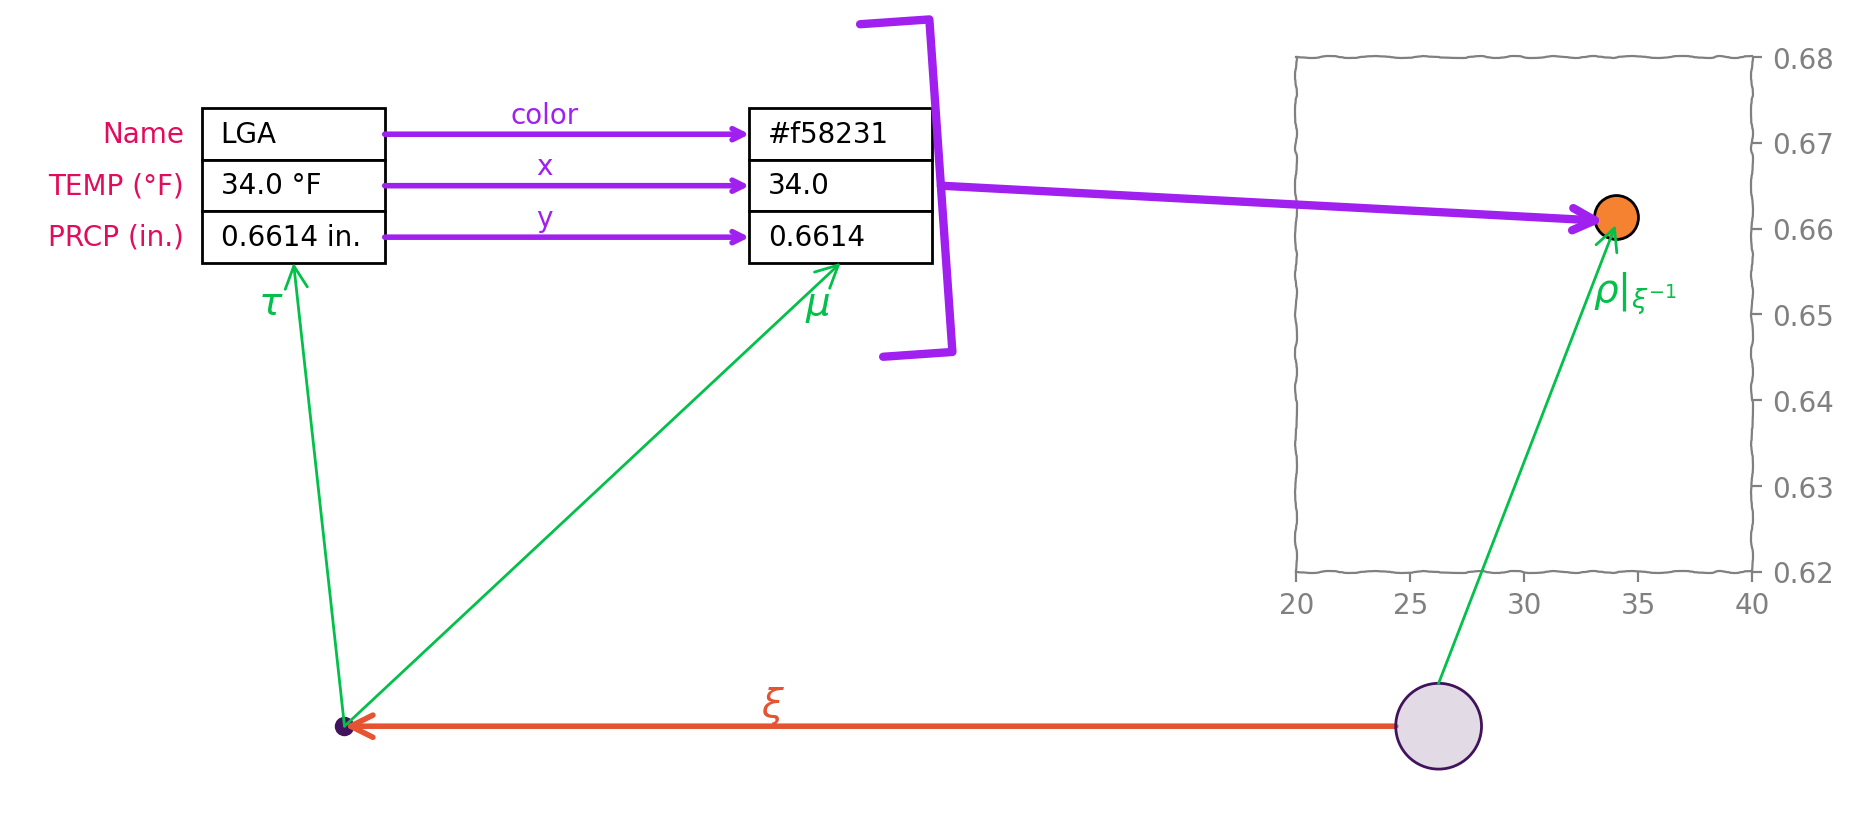
\includegraphics[width=1\columnwidth]{full_scatter.png}
  \caption{This simple $\vmarkc$ assembles a circular visual element that is the color specified in $\vsection(\dbasepoint)$ and is at the intersection specified in $\vsection(\dbasepoint)$ \label{fig:construction:q} \note{much better labeling, include semantic labeling, make everything bigger}}
\end{figure}
As shown in \autoref{fig:construction:q}, a set of  $\vchannel$ functions individually convert the values in the data record to visual components. Then the $\vmark$ function combines these visual encodings to produce a graphic section \gsection. When this section is evaluated on the graphic space associated with the data $\gsection(\vindexpre(\dbasepoint))$, it produces a blue circular marker at the intersection of the x and y positions listed in \vsection. The composition rule in \autoref{eq:construction:q:fabrication} means that developers can implement $\vmark$ as drawing circles or can implement a $\vmark$ that draws arbitrary shapes, and then provide different $\vchannel$ adapters, such as one that specifies that the shape is a circle.

\subsubsection{Compositor Verification}
\label{sec:construction:q:verification}
An advantage of factoring out encoding and verification, as discussed in \autoref{sec:construction:nu:verification}, is that the responsibility of the compositor can be scoped to translating measurable components into visual elements.
\begin{equation}
  \label{eq:construction:q:validate}
  \begin{tikzcd}[row sep=huge]
    \cgamma{\dbasec}{\vtotalc^{a}\times \vtotalc^{b}}
    \arrow[rr, "\vmarkc_{ab}", color=artist]
    \arrow[d, "\pi_a"', color=total] &  &  \imartistsub{ab}{\gbasec}{\gtotalc}
    \arrow[d, "\measurec\restriction_a \circ \extractmc_{ab}", color=monoid]  \\
   \cgamma{\dbasec}{\vtotalc^{a}}
   \arrow[rr, "\simeq", dotted] &  &
   {\textcolor{set}{Hom}(\dbasec, \measurec^{a})}  \\
    \cgamma{\dbasec}{\vtotalc^{a}\times \vtotalc^{c}}
    \arrow[rr, "\vmarkc_{ac}", color=artist]
    \arrow[u, "\pi_a", color=total]  &  &  \imartistsub{ac}{\gbasec}{\gtotalc}
    \arrow[u, "\measurec\restriction_a \circ \extractmc_{ac}"', color=monoid]
   \end{tikzcd}
\end{equation}
As illustrated in \autoref{eq:construction:q:validate}, a compositor is valid if there is an isomorphism between the actual outputted measured visual component and the expected measurable component that is the input. One way of verifying that a compositor is consistent is by verifying that it passes through one encoding even while changing others. For example, when $\vmark_{ab}=\vmark_{ac}$ then the output should differ in the same measurable components as $\vsectionc_{ab}$ and $\vsection_{ac}$.

A compositor function \vmark\ is equivariant if the renderer output changes in a way equivariant to the data transformation defined in \autoref{sec:artist:equivariant:data}. This means that a change in base space $\dfunch_{\dtotalc}$ should have an equivalent change in visual element base space. This means that there should be no change in visual measurement
\begin{equation}
  \label{eq:construction:q:verification:base}
  \vsectionc(\dfunchc_{\dbasec}(\dbasepointc^{\prime})) = \extractmc(\vmarkc(\vsectionc)(\dfunch_{\dbasec}(\vindexprec^{\dbasepointc}))) = \measurec_{\dbasepointc}
\end{equation}
As discussed in \autoref{fig:artist:equivariance}, the change in base space may induce a change in locations of measurements relative to each other in the output; this can be verified via checking that all the measurements have not changed relative to the original positions $\measurec_{\dbasepoint} = \measurec_{\dbasepointc^{\prime}}$ and through separate measurable variables that encode holistic data properties, such as orientation or origin.

The compositor function is also expected to be equivariant with respect to changes in data and measurable components
\begin{equation}
  \label{eq:construnction:q:verify:base}
  \dfunctc_{\vtotalc}(\vsectionc(\dbasepointc)) = \dfunctc_{\measurec}(\vmarkc(\vsectionc(\dbasepointc)))
\end{equation}
which means that any change to a measurable component input must have a measurably equivalent change in the output. As illustrated in \autoref{fig:artist:equivariance}, the compositor $\vmarkc$ is expected to assemble the measurable components such that base space changes, for example transposition, are reflected in the output; faithfully pass through equivariant measurable components, such as scaled colors; and ensure that both types of transformations, here scaling and transposition, are present in the final glyph.

\subsection{Implementing the Artist}
Since the artist is a family of functions in the homset between sheaves (\autoref{eq:atct:sheaves:homset}) the isomorphism allows for the specification of the transformation from data as a combination of functions over different spaces:

\begin{equation}
  \label{eq:construction:artist:path}
\begin{tikzcd}[row sep=2.5em, column sep=1.5em]
  \cgamma{\dbasec}{\dtotalc}
  \arrow[rr, "\vchannelc^{\dbasec}", color=artist]
  \arrow[rrrr, "\vartistc^{\dbasec}", bend left, color=artist]
  \arrow[dd, "\vindexpullc"', color=functor]
  \arrow[rrrrdd, "\vartistc", color=artist, pos=.2] &  &
  \cgamma{\dbasec}{\vtotalc}
  \arrow[rrdd, "\vmarkc", color=artist]
  \arrow[rr, "\vmarkc^{\dbasec}", color=artist]
  \arrow[dd, "\vindexpullc", color=functor, pos=.2] &  & \imartist{\dbasec}{\vindexpushc\gtotalc}  \\
   & & & & \\
  \cgamma{\gbasec}{\vindexpullc\dtotalc}
  \arrow[rr, "\vchannelc^{\gbasec}", color=artist]
  \arrow[rrrr, "\vartistc^{\gbasec}", bend right, color=artist] & &
  \cgamma{\gbasec}{\vindexpullc\vtotalc}
  \arrow[rr, "\vmarkc^{\gbasec}", color=artist] &  &
  \imartist{\gbasec}{\gtotalc}
  \arrow[uu, "\vindexpushc"', color=functor]
\end{tikzcd}
\end{equation}
This means that an artist over data space $\vartist_{\dbase}: \dsection \mapsto \vindexpush \gsection$, an artist over graphic space $vartist_{\gbase}: \vindexpull \dsection \mapsto \gsection$, and an artist $\vartist: \dsection \mapsto \gsection$ are equivalent such that:
\begin{equation*}
  \begin{split}
  & \dsection(\dbasepoint) = \vindexpull\dsection(\gbasepoint)  \\
   & \implies
  \vartist_{\dbase}(\dsection(\dbasepoint)) = \vartist_{\gbase}(\vindexpull\dsection(\gbasepoint)) = \vartist(\dsection(\dbasepoint))\\
  & \implies \vindexpush\gsection(\gbasepoint) = \gsection(\gbasepoint)
  \end{split}
\end{equation*}
when $\vindex(\gbasepoint) = \dbasepoint$. This equivalence allows a  developer to connect transformations over data space, denoted with a subset $\dbase$, with transformations over graphic space $\gbase$, using $\vindexpushc$ and $\vindexpullc$ adaptors.This allows developers to for example connect transformers that transform data on a line to a color in data space, but build a line compositing function that dynamically resamples what is on screen in graphic space.


\section{Discussion: Feasibility as Design Spec}
\label{sec:discussion}

The framework specified in \autoref{sec:artist} and \autoref{sec:construction} describes how to build structure preserving visualization components, but it is left to the library developer to follow these guidelines when building and reusing components. In this section, we introduce a toy example of building an artist out of the components introduced in \autoref{sec:construction} to illustrate how components that adhere to these specifications are maintainable, extendible, scalable, and support concurrency.

\begin{figure}[H]
  \centering
  \subfloat[]{
    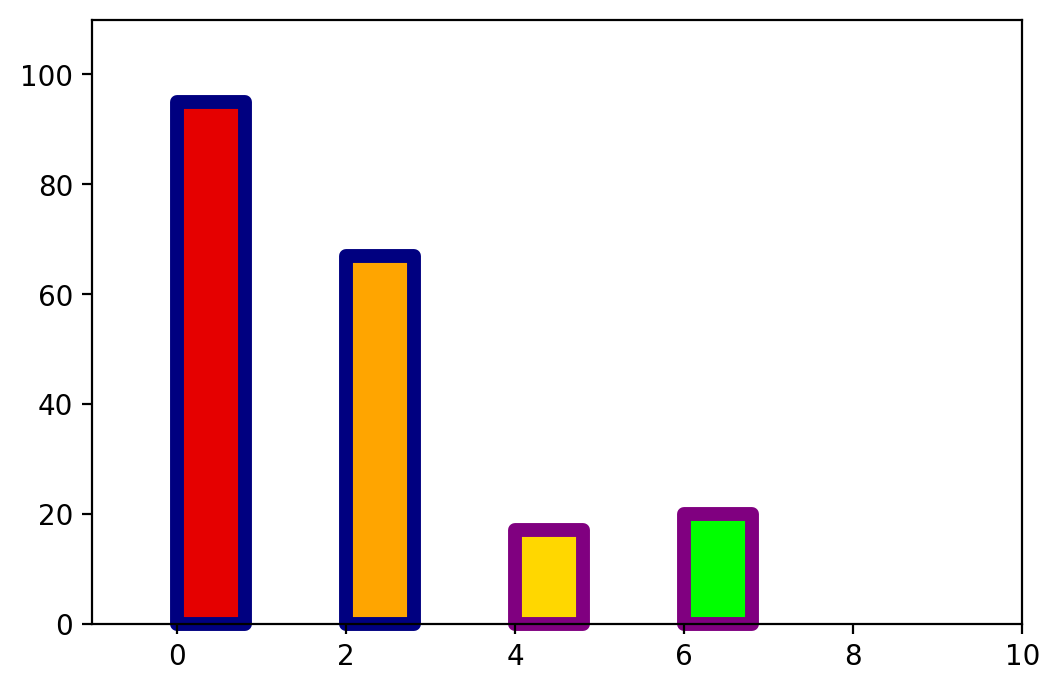
\includegraphics[width=.45\columnwidth]{bar.png}
  \label{fig:discussion:vbar}}
  \subfloat[]{
    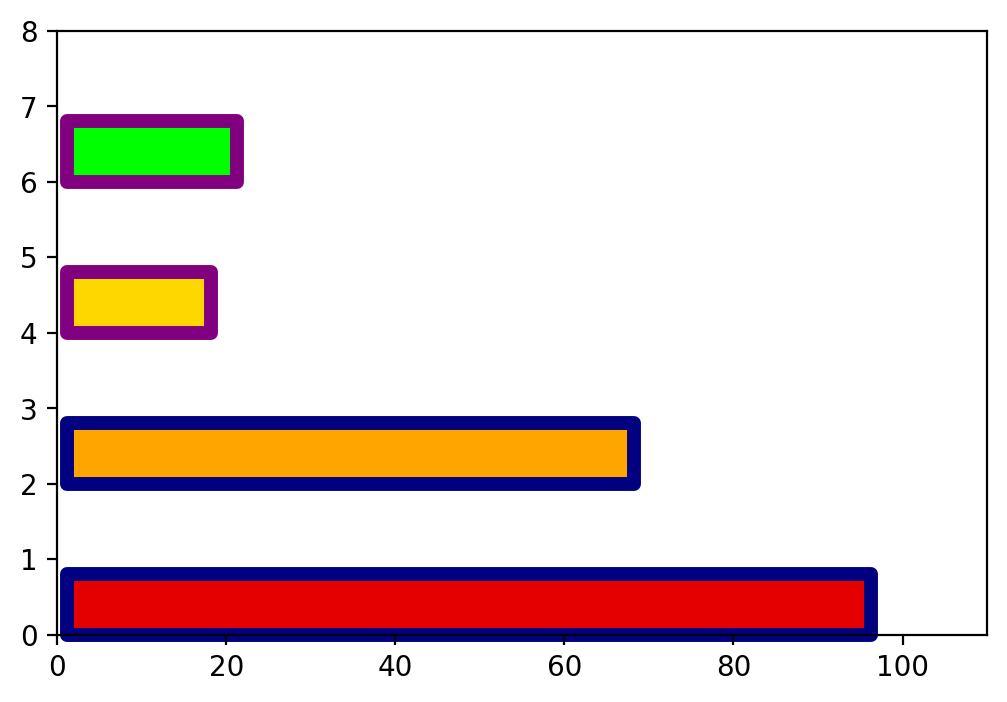
\includegraphics[width=.45\columnwidth]{barh.png}
  \label{fig:discussion:hbar}
  }
  \label{fig:discussion:bar}
\end{figure}

Specially, we introduce artists for building the graphical elements shown in \autoref{fig:discussion:bar} because it is a visualization type that allows us to demonstrate composability and multivariate data encoding. We build our visualization components by extending the Python visualization library Matplotlib's artist\footnote{Matplotlib artists are our artist's namesake}\cite{hunterMatplotlib2DGraphics2007,hunterArchitectureOpenSource} to show that components using this model can be incorporated into existing visualization libraries iteratively. While the architecture specified in \autoref{sec:construction} can be implemented fully functionally, we make use of objects to keep track of parameters passed into artists. In this toy example, the small composable components allow for more easily verifying that each component does its transformation correctly before assembling them into larger systems.

\subsection{Bundle Inspired Data Containers}
\begin{table}[H]
  \centering
\begin{tabular}{|lcl|}
  \hline \\
   fruit &  calories &  juice \\
  \hline\\
    apple &        95 &   True \\
   orange &        67 &   True \\
  lemon &        17 &  False \\
      lime &        20 &  False \\
  \hline
\end{tabular}
\label{tab:discussion:data}
\end{table}
We construct a toy dataset with a discrete $\dbase$ of 4 points and a fiber space of $\dfiber=\{apple,\, orange,\, lemon\}\times \mathbb{Z}^{+} \times \{\texttt{True}, \texttt{False}\}$. We thinly wrap \autoref{tab:discussion:data} in an object so that the common data interface function is that $\tau = \texttt{DataContainerObject.query}$.
\begin{minted}{python}
  class FruitFrameWrapper:
    def query(self, data_bounds, sampling_rate):
      # local sections are a list of
      # {field: local_batch_of_values}
      return local_sections
\end{minted}

This interface provides a uniform way of accessing subsets of the data, which are local sections. The motivation for a common data interface is that it would allow the artist to talk to different common python data containers, such as numpy\cite{harris2020array}, pandas\cite{jeff_reback_2020_3715232}, xarray \cite{hoyer2017xarray}, and networkx\cite{HagbergExploringNetwork2008}. Currently, data stored in these containers must be unpacked and converted into arrays and matrices in ways that either destroy or recreate the structure encoded in the container. For example a pandas data frame must be unpacked into its columns before it is sent into most artists and continuity is implicit in the columns being the same length rather than a tracked base space $\dbase$. Because it is more efficient to work with the data in column order, we often project the fiber down into individual components. As shown in \autoref{eq:atct:fiber_product}, we can verify that this projection is correct by checking that the values at the index are the same regardless of the level of decomposition.

\subsection{Component Encoders}
To encode the values in the dataset, we enforce equivariance by writing $\vchannel$ encoders that match the structure of the fields in the dataset. For example, the fruit column is a nominal measurement scale. Therefore we implement a position encoder that respects permutation $\dfunch$ transformations. The most simple form of this $\vchannel$ is a python dictionary that returns an integer position, because Matplotlib's internal parameter space expects a numerical position type.
\begin{minted}{python}
  def position_encoder(val):
    return {'apple': 0, 'orange': 2, 'lemon': 4, 'lime': 6}[val]
\end{minted}
As mentioned in \autoref{eq:construction:nu:fabrication}, the encoders can be composed up. For example, the compositor $\vchannel$ may need the position to be converted to screen coordinates. Here the screen coordinate $\vchannel$ is a method of a Matplotlib axes object; a Matplotlib axes is akin to a container artist that holds all information about the sub artists plotted within it.
\begin{minted}{python}
def composite_x_transform(ax, nu):
    return lambda x: ax.transData.transform(
            (position_encoder(x), 0))[0]
\end{minted}
This encoder returns a function that is \texttt{transData.transform} $\vchannel_{transData}$ composed with the position encoder $\vchannel_{position}$ and takes as input a record to be encoded. As with the position encoder, the transData encoder respects permutation transforms because it returns reals; therefore the composite encoder respects permutation transforms. In this model, developers implement $\vchannel$ encoders that are explicit about which $\dfunc_{\vtotal}$ they support. Writing semantically correct encoders is also the responsibility of the developer and is not addressed in the model. For example \mintinline{python}{fruit_encoder = lamda x: {'apple': green, 'orange':'yellow', 'lemon':'red', 'lime':'orange'}} is a valid color encoding with respect to permutation, but none of those colors are intuitive to the data. It is therefore left to the user, or domain specific library developer, to choose $\vchannel$ encoders that are appropriate for their data.

\subsection{Graphic Compositors}
After converting each record into an intermediate visual component $\vsection$, the set of visual records is passed into $\vmarkc$. Here the $\vmarkc$ includes one last encoder, as illustrated in \autoref{eq:construction:q:fabrication}, that assembles the independent visual components into a rectangle. This $\vchannel$ is inside the $\vmarkc$ to hide that library preferred format from the user. It is called \texttt{qhat} to indicate that this is the $\vartist^{\dbase}$ path in \autoref{eq:construction:artist:path}.  This means that the parameters are constructed in data space $\dbase$ and this function returns a pushed forward $\vindexpush\gsection$.

\begin{minted}{python}
   def qhat(position, width, length, floor, facecolor, edgecolor, linewidth, linestyle):
        box = box_nu(position, width, length, floor)
        def fake_draw(render, transform=mtransforms.IdentityTransform()):
            for (bx, fc, ec, lw, ls) in zip(box, facecolor, edgecolor, linewidth, linestyle):
                gc = render.new_gc()
                gc.set_foreground((ec.r, ec.g, ec.b, ec.a))
                gc.set_dashes(*ls)
                gc.set_linewidth(lw)
                render.draw_path(gc=gc, path=bx, transform=transform, rgbFace=(fc.r, fc.g, fc.b, fc.a))
        return fake_draw
\end{minted}
The function \texttt{fake\_draw} is the analog of $\vindexpush\gsection$. This function builds the rendering spec through the renderer API, and this curried function is returned. The transform here is required for the code to run, but is set to identity meaning that this function directly uses the output of the position encoders. The curried $\texttt{fake\_draw} \approx \vindexpush \gsection$ is evaluated using a renderer object. In our model, as shown in \autoref{eq:artist:inout:diagram}, the renderer is supposed to take $\gsection$ as input such that $renderer(\gsection) = visualization$, but here that would require an out of scope patching of the Matplotlib render objects.

One of the advantages of this model is that it allows for succinctly expressing the difference between two very similar visualizations, such as \autoref{fig:discussion:vbar} and \autoref{fig:discussion:hbar}. In this model, the horizontal bar is implemented as a composition of a $\vchannel$ that renames fields in $\vsection_{barh}$ and the $\vmark$ implementation for the horizontal bar.
\begin{minted}{python}
def qhat(length, width, position, floor, facecolor, edgecolor, linewidth, linestyle):
  return Bar.qhat(**BarH.bar_nu(length, width, position, floor, facecolor, edgecolor, linewidth, linestyle))
\end{minted}
This composition is equivalent to $\vmark_{barh} = \vmark_{bar} \circ \vchannel_{vtoh}$, which is an example of \autoref{eq:construction:q:fabrication}. These functions can be further added together, as described in \autoref{sec:artist:operators} to build more complex visualizations.

\subsection{Integrating Components into an Existing Library}
The $\vchannel$ and $\vmark$ are wrapped in a container object that stores the $\vartist = \vmark \circ \vchannel$ composition and a method for computing the $\vsectionc$.
\begin{minted}{python}
  class Bar:
    def compose_with_nu(self, pfield, ffield,
          nu, nu_inv:):
        # returns a new copy of the Bar artist
        # with the additional nu that converts
        # from a data (F) field value to a
        # visual (P) field value
        return new

    def nu(self, tau_local): #draw
       # uses the stored nus to convert data
       # stored nus have F->P field info
      return mus

    @staticmethod
    def qhat(position, width, length, floor, facecolor, edgecolor, linewidth, linestyle):

        return fake_draw
\end{minted}

As shown in the \texttt{draw} method, generating a graphic section $\gsection$ is implemented as the composition of $\texttt{qhat} \approx \vmark$ and $\texttt{nu} \approx \vchannel$ applied to a local section of the sheaf $\texttt{self.section.query} \approx \dsection^{i}$ such  $\texttt{draw} \approx \vmarkc\circ\vchannelc\circ\dsectionc  = \vartistc\circ \dsectionc$. The $\vchannel$ and $\vmark$ functions shown here are written such that they can generate a visual element given a local section $\dsection\restriction_{\dbase^{i}}$ which can be as little or large as needed. This flexibility is a prerequisite for building scalable and streaming visualizations that may not have access to all the data.

This artist is then passed along to a shim artist that makes it compatible with existing Matplotlib objects (\autoref{sec:appendix:artist_shim}). This shim object is hooked into the Matplotlib draw tree to produce the vertical bar chart in \autoref{fig:discussion:vbar}. Using the Matplotlib artist framework means this new artist can be composed with existing artists, such as the ones that draw the axes and ticks. The example in this section is intentionally trivial to illustrate that the math to code translation is fairly straightforward and results in fairly self contained composable functions. A library applying these ideas, created by Thomas Caswell and Kyle Sunden, can be found at \url{https://github.com/matplotlib/data-prototype}. Further research could investigate building new systems using this model, specifically libraries for visualizing domain specific structured data and domain specific artists. More research could also explore applying this model to visualizing high dimensional data, particularly building artists that take as input distributed data and artists that are concurrent. Developing complex systems could also be an avenue to codify how interactive techniques are expressed in this framework.

\section{Conclusion}
The toy example presented in \autoref{sec:discussion} demonstrates that it is relatively straightforward to build working visualization library components using the construction described in \autoref{sec:construction}. Since these components are defined with single record inputs, they can be implemented such that they are concurrent. The cost of building a new function using these components is sometimes as small as renaming fields, meaning the new feature is relatively easy to maintain. These new components are also a lower maintenance burden because, by definition, they are designed in conjunction with tests that verify that they are equivariant.
These new components are also compatible with the existing library architecture, allowing for a slow iterative transition to components built using this framework.
The framework introduced in this paper is a marriage of the ways the graphic and data visualization communities approach visualization. The graphic community prioritizes \note{?} how input is translated to output, which is encapsulated in the artist $\vartist$. The data visualization community prioritizes the manner in which that input is encoded, which is encapsulated in the separation of stages $\vmark \circ \vchannel$. Formalizing that both views are equivalent $\vartist=\vmark \circ \vchannel$ gives library developers the flexibility to build visualization components in the manner that makes more sense for the domain without having to sacrifice the equivariance of the translation.

\appendices

\section{Summary}
\label{sec:appndix:summary}
The topological spaces and functions introduced throughout this paper are summarized here for reference.

\begin{table}[H]
  \centering
  {\renewcommand{\arraystretch}{1.2}
  \begin{tabular}{|r | c c c|}
    \hline
    &\textcolor{base}{point}/\textcolor{base}{openset}/\textcolor{base}{base space} & \textcolor{fiber}{fiber space} & \textcolor{total}{total space}\\
     &  location/subset/indices & record/fields &  dataset type\\
    \hline
   Data & $\dbasepointc \in \opensetc \subseteq \dbasec$ & $\delementc \in \dfiberc$ & \dtotalc\\
   Visual & $\dbasepointc \in \opensetc \subseteq \dbasec$  & $\velementc \in \vfiberc$ & \vtotalc\\
   Graphic & $\gbasepointc \in \opensetgc \subseteq \gbasec$ & $\gelementc \in \gfiberc$ & \gtotalc\\
   \hline
  \end{tabular}
  \caption{Topological spaces introduced in \autoref{sec:atct:fiber-bundles}}
  \label{tab:appendix:summary:objects}
  }
\end{table}

\begin{table}[H]
  \centering
  {\renewcommand{\arraystretch}{1.2}
  \begin{tabular}{|r | l l | }
    \hline
     & \textcolor{section}{section} & \textcolor{sheaf}{sheaf} \\
     & record at location & set of possible records for subset \\
     \hline
  Data & $ \cgamma{\dbasec}{\dtotalc} \ni \dsectionc: \dbase \textcolor{section}{\rightarrow} \dfiberc$ & $\sheafc_{\dbasec, \dtotalc}: \opensetc \rightarrow \cgamma{\opensetc}{\dtotalc\restriction_{\opensetc}}$\\
  Visual &  $\cgamma{\dbasec}{\vtotalc} \ni \vsectionc: \dbase \textcolor{section}{\rightarrow} \vfiberc$ & $\sheafc_{\dbasec, \vtotalc}: \opensetc \rightarrow \cgamma{\opensetc}{\vtotalc\restriction_{\opensetc}}$\\
  Graphic &    $\cgamma{\gbasec}{\gtotalc} \ni \gsectionc: \gbase \textcolor{section}{\rightarrow} \gfiberc$ &  $\sheafc_{\gbasec, \gtotalc}: \opensetgc \rightarrow \cgamma{\opensetc}{\gtotalc\restriction_{\opensetgc}}$ \\
  \hline
  \end{tabular}
  \caption{Functions that associate topological subspaces with records, discussed in \autoref{sec:atct:fb:sections} and \autoref{sec:atct:sheaves}}
  \label{tab:appendix:summary:datafunctions}
  }
\end{table}

\begin{table}[H]
  \centering
  {\renewcommand{\arraystretch}{1.2}
  \begin{tabular}{|r|l|}
    \hline
      axiom & applied to datasets and indexes \\
    \hline
     presheaf & given $\textcolor{base}{index_1} \subset \textcolor{base}{index_2}$:\\
        & $\exists\;\textcolor{section}{dataset}[\textcolor{base}{index_2}]$\\
      & $\Rightarrow \textcolor{section}{dataset}[\textcolor{base}{index_2}][\textcolor{base}{index_1}] = \textcolor{section}{dataset}[\textcolor{base}{index_1}]$\\
     &  $\exists\;\textcolor{section}{dataset}[\textcolor{base}{index_1}] \nRightarrow \exists\;\textcolor{section}{dataset}[\textcolor{base}{index_2}]$\\
     &\\
    \hline
    locality & $\textcolor{section}{dataset^1}[\textcolor{base}{i}] = \textcolor{section}{dataset^2}[\textcolor{base}{i}]\;\forall\; \textcolor{base}{i}\in \textcolor{base}{index}\;$ \\
     & $\Rightarrow \textcolor{section}{dataset^1}=\textcolor{section}{dataset^2}$ \\
    \hline
    gluing & $\textcolor{base}{i}=\textcolor{base}{j}$ and $\textcolor{section}{dataset^1}[\textcolor{base}{i}] = \textcolor{section}{dataset^2}[\textcolor{base}{j}]$ \\
     & $\textcolor{section}{dataset^3}\coloneq  \textcolor{section}{dataset^1}[\textcolor{base}{:i}]  \oplus \textcolor{section}{dataset^2}[\textcolor{base}{j:}]$ \\
\hline
  \end{tabular}
  \caption{Presheaf and sheaf constraints implemented by structure preserving data containers, discussed in \autoref{sec:atct:sheaves}}
  \label{tab:appendix:summary:sheaves}
  }
\end{table}

\begin{table}[H]
  \centering
  {\renewcommand{\arraystretch}{1.2}
  \begin{tabular}{|r | l  l |}
\hline
& function & constraint\\
\hline
 \gbasepointc\ to \dbasepointc& $ \vindexc: \opensetgc \rightarrow \opensetc$ & for $\gbasepointc \in \opensetgc$ exists $\dbasepointc \in \opensetc$ \\
 & & s.t. $\vindexc(\gbasepointc) = \dbasepointc$\\
 graphic for \dbasepointc & $ \vindexpushc \gsectionc: \opensetc \rightarrow \vindexpushc\gtotalc\restriction_{\opensetc}$ & $\vindexpushc\gsectionc(\dbasepointc)(\gbasepointc) = \gsectionc(\gbasepointc)$ \\
 record for \gbasepointc & $\vindexpullc\dsectionc: \opensetgc \rightarrow  \vindexpullc\dtotalc\restriction_{\opensetgc}$ & $\vindexpullc\dsectionc(\gbasepointc)=\dsectionc(\vindexc(\gbasepointc)) = \dsectionc(\dbasepointc)$  \\
\hline
  \end{tabular}
  \caption{Functors between graphic and data indexing spaces  \autoref{sec:atct:xi}}
  \label{tab:appendix:summary:transport}
  }
\end{table}



\begin{table}[H]
\centering
{\renewcommand{\arraystretch}{1.2}
\begin{tabular}{|r|l|l|}
  \hline
  changes & function & constraints, for all $\dbasepointc \in \opensetc$ \\
  \hline
  index & $\dfunchc: \opensetc \rightarrow \opensetc^{\prime}$ &   $\dsectionc(\dbasepointc) = \dsectionc(\dfunchc(\dbasepointc^{\prime})) = \dfuncpullc \dsectionc(\dbasepointc^{\prime})$ \\
  & & \\
  record  & $\dfunctc: \cgamma{\opensetc^{\prime}}{\dfuncpullc\dtotalc\restriction_{\opensetc}}$ &  $\lim\limits_{x\rightarrow \dbasepointc}\dfunctc(\dsectionc(x)) = \dfunctc(\dsectionc(\dbasepointc))$
  \\
  & $\textcolor{white}{\dfunct: } \rightarrow \cgamma{\opensetc^{\prime}}{\dfuncpullc\dtotalc\restriction_{\opensetc}}$ &
  \\
  & $\dfunctc: \dfiberc \rightarrow \dfiberc$ &  $\dfunctc(\dsectionc(\dbasepointc)) \in \dfiberc$  \\
  & & $\dfunctc(id_{\dfiberc}(\dsectionc(\dbasepointc))) = id_{\dfiberc}(\dfunctc(\dsectionc(\dbasepointc)))$\\
  & & $\dfunctc(\dfunctc(\dsectionc(\dbasepointc))) = (\dfunctc\circ\dfunctc)(\dsectionc(\dbasepointc))$\\
  \hline
\end{tabular}
\caption{Functions $\dfunc=(\dfunchc, \dfunctc)$ for modifying data records. Equivalent constructions can be applied to elements in visual and graphic sheaves, and these functions are distinguished through subscripts $\dfunc_{\dtotal}$, $\dfunc_{\vtotal}$ and $\dfunc_{\gtotal}$}
\label{tab:appendix:summary:datamod}
}
\end{table}

\begin{table}[H]
  \renewcommand{\arraystretch}{1.2}
  \begin{tabular}{|lll|}\hline
      scale & operators & sample constraint \\ \hline
      nominal & $=,\neq$ &  $\dsectionc(\dbasepointc_1) \neq \dsectionc(\dbasepointc_2)\implies \dfunctc (\dsectionc(\dbasepointc_1)) \neq\dfunctc(\dsectionc(\dbasepointc_2))$\\
      ordinal & $<, \leq, \geq, >$ &  $\dsectionc(\dbasepointc_1) \leq \dsectionc(\dbasepointc_2) \implies \dfunctc (\dsectionc(\dbasepointc_1)) \leq \dfunctc(\dsectionc(\dbasepointc_2)$) \\
      interval & $+, -$ &  $\dfunctc(\dsectionc(\dbasepointc) + C) = \dfunctc(\dsectionc(\dbasepointc)) + C$ \\
      ratio & $*,/$ &  $\dfunctc(\dsectionc(\dbasepointc) * C) = \dfunctc(\dsectionc(\dbasepointc))*C $\\ \hline
  \end{tabular}
  \caption{The record transformer $\dfunctc$ must satisfy the constraints listed in \autoref{tab:appendix:summary:datamod} and $\dfunctc$ must also respect the mathematical structure of $\dfiber$. This table lists examples of $\dfunct$ preserving one of the binary operators that are part of the definition of each of the Steven's measurement scale types\cite{stevensTheoryScalesMeasurement1946}}. A full implementation would ensure that all operators that are defined as part of of $\dfiber$ are preserved.
  \label{tab:appendix:summary:stevens}
\end{table}

\begin{table}[H]
  \centering
  {\renewcommand{\arraystretch}{1.2}
\begin{tabular}{|r|l|l|}
  \hline
      & function & constraints \\
  \hline
  \textcolor{artist}{artist} & $\vartistc: \cgamma{\dbasec}{\dtotalc} \rightarrow \imartist{\gbasec}{\gtotalc}$ &  \\
  Data to Graphic  &  $\imartist{\gbasec}{\gtotalc} \subset \cgamma{\gbasec}{\gtotalc}$ & $\vindexc(\gbasec) = \dbasec$\\
  & & \\
  \hline
  Encode
    & & \\
           & & \\
  \hline
  Decompose & & \\
              && \\
  \hline
\end{tabular}
\caption{artist, verification functions, and construction $\vartist = \vmarkc \circ \nu$ introduced in \autoref{sec:artist}, and \autoref{sec:construction}}
\label{tab:appedendix:summary:artist}
}
\end{table}


\note{color}
\begin{table}[H]
  \centering
  {\renewcommand{\arraystretch}{1.2}
\begin{tabular}{|r|l|l|}
  \hline
      & function & constraint \\
  \hline
  \textcolor{artist}{artist} & $\vartist: \Gamma(\dbase, \dtotal) \rightarrow \Gamma(\gbase, \gtotal)$ &  \\
  \hline
  \textcolor{functor}{lookup} & $\vindex: \gbase\rightarrow \dbase$  &  \\
  \hline
  \textcolor{artist}{encoders} & $\vchannel: \Gamma(\dbase, \dtotal) \rightarrow \Gamma(\dbase, \vtotal) $  & \\
  \hline
  \textcolor{artist}{compositor} & $\vmark: \Gamma(\dbase,\vtotal) \rightarrow \Gamma(\gbase, \vtotal)$ &  \\
  \hline
\end{tabular}
\caption{artist, verification functions, and construction $\vartist = \vmarkc \circ \nu$ introduced in \autoref{sec:artist}, and \autoref{sec:construction}}
\label{tab:appendix:summary:artist}
}
\end{table}

\section{Trivial and non-trivial bundles}
\label{sec:appendix:bundle_triviality}

Generally, the distinguishing factor between a trivial bundle and a non-trivial bundle are how they are decomposed into local trivializations:
\begin{LaTeXdescription}
  \item[\textit{trivial bundle}] is directly isomorphic to $\dbasec\times\dfiberc$. For any choice of cover of $\dbasec$ by overlapping opensets, we can choose local trivializations such that all transition maps are identity maps.
  \item[\textit{non-trivial bundle}] can not be constructed as $\dbasec\times\dfiberc$. For any choice of local trivializations, there is at least one transition map that is not an identity \cite{hatcherAlgebraicTopology2002}.
\end{LaTeXdescription}


\begin{figure}[H]
  \includegraphics[width=1\columnwidth]{transition_maps.pdf}
  \caption{The cylinder is a trivial fiber bundle; therefore it can be decomposed into local trivializations that only need identity
  maps to glue the trivializations together. The mobius band is a non-trivial bundle; therefore it can only be decomposed into trivializations where at least one transition map is not an identity map. }\label{fig:cyl_mob_bundles}
\end{figure}

In the example in Figure~\ref{fig:cyl_mob_bundles}, we use arrows $\uparrow$ to denote fiber alignments. In the cylinder case the fibers all point in the same direction, which illustrates that they are equal $\uparrow=\uparrow$. In the Möbius band case, while the fibers in an arbitrary local trivialization are equal $\uparrow=\uparrow$, the fibers at the twist are unequal but isomorphic $\uparrow \cong \downarrow$. The cylinder and mobius band can be decomposed to the same local trivializations, for example the fiber bundles in \autoref{fig:atct:fb} In the cylinder case, the fibers in the overlapping regions of the trivializations are equal $\dfiber_0\restriction_{\openset_1\cap\openset_2} = \dfiber_{1}\restriction_{\openset_1\cap\openset_2}$; therefore the transition maps at both intersections map the values in the fiber to themselves $\delement\rightarrow\delement$ . In the Möbius band case, while $\dfiber_0\restriction_{(2\pi/5-\varepsilon, 2\pi/5+\varepsilon)}\to\dfiber_1\restriction_{(2\pi/5-\varepsilon, 2\pi/5+\varepsilon)}$ can be chosen to be an identity map, the other transition map component $\dfiber_0\restriction_{(-\varepsilon,\varepsilon)}\to\dfiber_1\restriction_{(-\varepsilon,\varepsilon)}$ has to flip any section values. For example given  $\dfiber_{0}=\uparrow$ and $\dfiber_{1}=\downarrow$, the transition map $\delement \mapsto -\delement$ maps each point from one fiber to the other $\uparrow \mapsto \downarrow$ such that any sections remain continuous even though the fibers point in opposite directions.


\section{Internal Library Specification}
As mentioned in \autoref{sec:construction:vtotal}, the internal types of visualization libraries can be defined using this model, which creates a consistent standard for developers writing new functions to target. These are the formal specifications of various aesthetic parameters in Matplotlib.

\label{tab:appendix:library_spec}
\begin{table}[H]
  \centering
  \renewcommand{\arraystretch}{2}
  \begin{tabulary}{\columnwidth}{|l|L|l|}\hline
   \(\bm{\vchannel_{i}}\)    & \(\bm{\vsection_{i}}\)  & \(\bm{codomain(\vchannel_{i}) \subset \vfiber_{i}}\)  \\ \hline
  position                    & x, y, z, theta, r      & \(\mathbb{R}\)   \\ \hline
  size                        & linewidth, markersize  & \(\mathbb{R}^{+}\)  \\ \hline
  shape                       & markerstyle            & \(\{f_{0}, \ldots, f_{n}\}\)\\ \hline
  color                       & color, facecolor, markerfacecolor, edgecolor  & \(\mathbb{R}^{4}\) \\ \hline
  \multirow{2}{*}{texture}    & hatch      & \(\mathbb{N}^{10}\)\\\cline{2-3}
                              & linestyle    & \((\mathbb{R}, \mathbb{R^+}^{n, n\%2=0})\) \\ \hline
  \end{tabulary}
  \caption{Some of the $\vfiber$ components of the $\vtotal$ bundles in Matplotlib components}
  \label{tab:math:artist:mpl:fiber}
\end{table}

\pagebreak
\section{Matplotlib Compatibility}
\label{sec:appendix:artist_shim}

As mentioned in \autoref{sec:discussion}, one advantage of using this type of
functional categorical approach to software design is that we can develop new
components that can be incorporated into the existing code base. For matplotlib,
we can use these functional artists by wrapping them in a very thin compatibility
layer shim so that they behave like existing artists.

\begin{minted}{python}
  class GenericArtist(martist.Artist):
      def __init__(self, artist:TopologicalArtist):
          super().__init__()
          self.artist = artist

      def compose_with_tau(self, section):
          self.section = section

      def draw(self, renderer, bounds, rate):
          for tau_local in self.section.query(bounds, rate):
              mu = self.artist.nu(tau_local)
              rho = self.artist.qhat(**mu)
              output = rho(renderer)
  \end{minted}

\section*{Acknowledgment}
\note{Acknowledge all the actual people}
The authors would like to thank the anonymous reviewers who gave constructive feedback on an earlier version of this paper. The authors are also grateful to  the various Matplotlib and Napari contributors, particularly Juan Nunez-Iglesias, and Nicolas Kruchten for their valuable feedback from the library developer perspective.

Hannah is also very grateful to Nicolas for the suggestion of augmented notation and to the nlab and wikipedia contributors who wrote clear explanations of many of the topics discussed in this paper.

This project has been made possible in part by grant number 2019-207333 and \note{Cycle 3 grant number} Chan Zuckerberg Initiative DAF, an advised fund of Silicon Valley Community Foundation


% Can use something like this to put references on a page
% by themselves when using endfloat and the captionsoff option.
\ifCLASSOPTIONcaptionsoff
  \newpage
\fi

% trigger a \newpage just before the given reference
% number - used to balance the columns on the last page
% adjust value as needed - may need to be readjusted if
% the document is modified later
%\IEEEtriggeratref{8}
% The "triggered" command can be changed if desired:
%\IEEEtriggercmd{\enlargethispage{-5in}}

% references section

\printbibliography

% biography section
% If you have an EPS/PDF photo (graphicx package needed) extra braces are
% needed around the contents of the optional argument to biography to prevent
% the LaTeX parser from getting confused when it sees the complicated
% \includegraphics command within an optional argument. (You could create
% your own custom macro containing the \includegraphics command to make things
% simpler here.)
%\begin{IEEEbiography}[{\includegraphics[width=1in,height=1.25in,clip,keepaspectratio]{mshell}}]{Michael Shell}
% or if you just want to reserve a space for a photo:

%\begin{IEEEbiography}{Michael Shell}
%\end{IEEEbiography}

% if you will not have a photo at all:
\begin{IEEEbiographynophoto}{Hannah Aizenman}
Biography text here.
\end{IEEEbiographynophoto}

\begin{IEEEbiographynophoto}{Thomas Caswell}
  Biography text here.
\end{IEEEbiographynophoto}
% insert where needed to balance the two columns on the last page with
% biographies
%\newpage

\begin{IEEEbiographynophoto}{Michael Grossberg}
Biography text here.
\end{IEEEbiographynophoto}

% You can push biographies down or up by placing
% a \vfill before or after them. The appropriate
% use of \vfill depends on what kind of text is
% on the last page and whether or not the columns
% are being equalized.

%\vfill

% Can be used to pull up biographies so that the bottom of the last one
% is flush with the other column.
%\enlargethispage{-5in}

% that's all folks
\end{document}
